\documentclass{article}
\input{../packages.tex}
\input{../commons.tex}
\usepackage{parskip}

\title{Analisi e Progettazione Algoritmi}
\author{Adrian Castro, Ilaria Battiston \thanks{Slides di Mauri}}
\date{Ottobre 2018}
\pagestyle{fancy}

\begin{document}

\maketitle

\lfoot{}
\cfoot{}
\rfoot{\thepage}

\newpage
\tableofcontents
\newpage
\section{Introduzione}

\subsection{Chiarimenti sul corso}

\begin{enumerate}
    \item Ricevimento U14 1010 1$^\circ$ piano;
    \item \href{mailto:zandron@disco.unimib.it}{zandron@disco.unimib.it};
    \item Modalità d'esame: \begin{enumerate}
        \item Scritto: esercizi + teoria;
        \item Verbalizzazione normale;
        \item Compitini: \begin{enumerate}
            \item 1o: esercizi;
            \item 2o: esercizi + teoria.
        \end{enumerate}
    \end{enumerate}
\end{enumerate}

\subsection{A grandi linee}

\subsubsection{Programmazione dinamica}
La programmazione dinamica è un metodo di risoluzione dei problemi che consiste nel trovare sotto-informazioni che poi verranno riutilizzate con il tempo. Il problema viene spezzato in parti, e si cerca di trovare una sotto-informazione che può essere sfruttata quando necessario. Efficiente in termini di spazio e tempo. 

Alcuni algoritmi hanno una soluzione intuitiva, ma che richiedono di ricalcolare tante volte la stessa cosa. Una soluzione può essere usare una \textbf{cache}, memoria dove vengono salvati i valori calcolati precedentemente. A questo punto, però, l'algoritmo è meno efficiente dal punto di vista dello \textbf{spazio}. Bisogna quindi capire in quali casi è opportuno attuare una tecnica del genere. 

La programmazione dinamica viene usata nei problemi di ottimizzazione e di decisione. Gli algoritmi di decisione devono saper rispondere a ogni tipo di input (es. esiste un cammino che collega due nodi?). 

Un altro problema è la ricerca: dato un input $x$, determinare una soluzione $S$ che rispetti le caratteristiche del problema. Deve esistere $S$ tale che esista un collegamento $(x,\ S)$. 

L'ottimizzazione associa a ogni soluzione il relativo costo e cerca la miglior soluzione possibile in base al costo minimo: $S^*\:|\:C(S^*) \leq C(S)$. \\
Bisogna considerare anche che alcune soluzioni non sono ammissibili.

\subsubsection{Programmazione reedy}
Il tipo di programmazione \textbf{greedy} (o \textbf{goloso}), viene usata per determinare la soluzione migliore tramite una serie di calcoli effettuati localmente, per esempio previsioni in base ai dati correnti. Non si conosce l'andamento dei dati nel futuro. \par
Una tecnica di programmazione \textbf{greedy} si basa sulla situazione attuale per capire cosa fare successivamente. \par
Esempio: problema del $travelling\ salesman$. La tecnica greedy continua a ridurre le possibilità di scelta, più avanti si va nell'algoritmo. Ciò significa che le scelte attuali di viaggio possono sembrare poco costose, ma poi magari ci si ritrova con le ultime scelte che hanno spese insostenibili. \par
In casi di questo tipo, un algoritmo \textbf{greedy} non è la scelta più adatta. Possiamo quindi fare la seguente osservazione:
\begin{definition}{Algoritmo Greedy}{greedy}
    Gli algoritmi di tipo greedy funzionano al meglio se tutti i pesi (o valori) delle scelte sono uguali a $1$.
\end{definition}
$$
\begin{tikzpicture}
    \matrix (m) [matrix of math nodes, row sep=2em,
    column sep=1em]{
    & & c_1 & & \\
    c_2 & & & & c_3 \\
    & c_4 & & c_5 & \\};
    \path[-stealth]
    (m-1-3) edge (m-2-1) % c1
            edge (m-2-5)
            edge (m-3-2)
            edge (m-3-4)
    (m-2-1) edge (m-2-5) % c2
            edge (m-2-5)
            edge (m-3-2)
            edge (m-1-3)
            edge (m-3-4)
    (m-2-5) edge (m-2-1) % c3
            edge (m-1-3)
            edge (m-3-4)
            edge (m-3-2)
    (m-3-2) edge (m-1-3) % c4
            edge (m-2-1)
            edge (m-2-5)
            edge (m-3-4)
    (m-3-4) edge (m-1-3) % c5
            edge (m-2-1)
            edge (m-2-5)
            edge (m-3-2);
\end{tikzpicture}
$$

Alcuni algoritmi sui grafi implementabili con uno dei due metodi di programmazione sono BFS, DFS, cammini minimi, problemi di flusso.
Quando nessun algoritmo è in grado di risolvere un problema in tempo accettabile (non esponenziale) si parla di NP-completezza.
\section{Ripasso di algoritmi}

\subsection{Risoluzione di algoritmi e tempi di esecuzione}
Un problema risoluzione di algoritmi rientra sempre in uno di tre casi:
\begin{enumerate}
	\item Problema risolvibile in modo efficiente;
	\item Problema risolvibile in modo non efficiente;
	\item Problema non risolvibile.
\end{enumerate}
Il metodo può essere iterativo o ricorsivo. Con il modo iterativo, una serie di operazioni sono ripetute più volte all'interno della stessa funzione, e lo sviluppo dell'algoritmo è intuitivo. Per ogni possibile input, la risposta ottenuta alla fine della sequenza di istruzioni dev'essere corretta. Alcuni esempi di algoritmi iterativi sono l'ordinamento tramite selection sort, insertion sort e bubble sort; altri sono la \textbf{ricerca dicotomica}, \textbf{ricerca del massimo e del minimo}.
\par Il tempo di esecuzione viene misurato in base al numero di istruzioni, utilizzando limiti asintotici. Valutare il tempo di esecuzione significa capire (asintoticamente) quante istruzioni vengono eseguite con un input di dimensione n, cioè 
$$T(n), n = |x|, x = input$$ 
Ogni algoritmo ha tre modi di rappresentarne il tempo, che indicano l'ordine di complessità di $f(n)$:
\begin{itemize}
	\item Caso migliore (numero minimo di istruzioni), $t(n)$ oppure $\Omega(f(n))$, che significa che la funzione è limitata inferiormente;
	\item Caso peggiore (numero massimo di istruzioni, garanzia sul tempo massimo), $T(n)$ oppure $O(f(n))$, che significa che la funzione è limitata superiormente;
	\item Caso medio (tempo medio di esecuzione in base al caso possibile più frequente), $T_m(n)$ oppure $\Theta(f(n))$, che significa che la funzione è compresa tra due limiti.
\end{itemize}

\subsection{Algoritmi iterativi}
Selection sort è l'algoritmo di sorting più semplice, che consiste nella ricerca lineare del minimo in un ciclo $for$. \par
\begin{algorithm}
	\caption{Selection sort iterativo}
	\label{alg:ssi}
	\begin{algorithmic}
		\Function{selection\_sort}{$A$}
		\For{$j \gets 1$ \textbf{to} (\Call{length}{$A$} - 1) \textbf{step} $1$}
		\For{$i \gets j$ \textbf{to} \Call{length}{$A$} \textbf{step} $1$}
		\State $min \sim A[i]$
		\EndFor
		\State \Call{scambia}{$A, j, min$}
		\EndFor
		\EndFunction
	\end{algorithmic}
\end{algorithm}
Il tempo di esecuzione sarebbe
$$\sum_{i=1}^{n}i + \sum_{i=1}^{n}i + 3(n - 1)$$
approssimabile a $\Theta(n^2)$.
\par Insertion sort è un algoritmo meglio funzionante rispetto a selection sort, rappresentabile come l'ordinamento di un mazzo di carte di cui $k$ ordinate, scoprendo una carta per volta. Ogni carta viene controllata e riposizionata in modo da avere un array di carte ordinate. \par
\begin{algorithm}
	\caption{Insertion sort iterativo}
	\label{is}
	\begin{algorithmic}
		\Function{insertion\_sort}{$A$}
		\For{$j \gets 2$ \textbf{to} \Call{length}{A} \textbf{step} $1$}
		\State $carta \gets A[i]$
		\While{$A[j] > carta \land j > 0$}
		\State $A[j + 1] \gets A[j]$
		\State $j \gets j - 1$
		\State $A[j + 1] \gets carta$
		\EndWhile
		\EndFor
		\EndFunction
	\end{algorithmic}
\end{algorithm}
Il tempo di esecuzione dipende dal numero di volte in cui $while$ è vero, cioè
$$4n + 3\sum_{i=2}^{n}t_wi$$
(con $t_wi$ numero di volte che viene eseguito $while$).
\begin{enumerate}
	\item Caso Migliore: array già ordinato, $\Theta(n)$.
	\item Caso Peggiore: array ordinato al contrario, $O(n^2)$
	\item Caso Medio: l'ordinamento richiede metà iterazioni di $while$, approssimato a $\Theta(n^2)$
\end{enumerate}

\subsection{Algoritmi ricorsivi}
Nonostante selection sort e bubble sort abbiano tempi computazionali generamente minori rispetto a selection sort, essi non sono ancora ottimizzati per input lunghi. \par
Gli algoritmi ricorsivi contengono funzioni che chiamano loro stesse con un input di dimensione minore rispetto all'originale, continuando a diminuirne le dimensioni fino ad arrivare al caso base (semplice). \par
\begin{algorithm}
	\caption{Ricerca del massimo ricorsivo}
	\label{alg:rmr}
	\begin{algorithmic}
		\Function{max\_ric}{$A, i, n$}
			\If{$i == n$}
				\State \Return i
				\Else
					\State \Call{max\_ric}{A[], i+1, n}
				\If{$A[i] > A[Rp]$}
					\State \Return i
				\Else
					\State \Return Rp
				\EndIf
			\EndIf
		\EndFunction
	\end{algorithmic}
\end{algorithm}
Il tempo di esecuzione può essere descritto in questo modo:
$$T(n) = \begin{cases}
	2 & se\ n = 1 \\
	3 + T(n - 1) & se\ n > 1
\end{cases}$$
L'equazione di ricorrenza viene risolta con tre possibili metodi:
\begin{enumerate}
	\item Metodo iterativo (dell'albero);
	\item Metodo di induzione;
	\item Metodo dell'esperto.
\end{enumerate}
Utilizzando questo metodo è possibile arrivare a un tempo asintotico di $\Theta(n)$. \par
Un altro algoritmo ricorsivo è la ricerca del $k$-esimo elemento della sequenza di Fibonacci. L'implementazione standard richiama la funzione su $(n - 1)$ e $(n-2)$. Il problema di questo algoritmo è l'elevata complessità computazionale, la quale cresce esponenzialmente (al contrario di altri come il fattoriale). \\
Il metodo più efficiente per Fibonacci è tramite la programmazione dinamica, salvando i risultati intermedi in memoria. \par

Merge sort è un popolare algoritmo di algoritmi ricorsivo che sfrutta la tecnica del divide-et-impera: divide il problema in uno o più sotto-problemi, usa la ricorsione per risolvere i sotto-problemi e ne combina le soluzioni. \par
\begin{algorithm}
	\caption{Merge sort ricorsivo}
	\label{alg:msr}
	\begin{algorithmic}
		\Function{MS}{$A[], I, F$}
			\State $m \gets (I + F) / 2$
			\State \Call{MS}{$A[], I, m$}
			\State \Call{MS}{$A[], m + 1, F$}
			\State \Call{Merge}{$A[], I, m, F$}
		\EndFunction
	\end{algorithmic}
\end{algorithm}
Questo algoritmo ha una parte iterativa (divide e combina) e una parte ricorsiva (impera) le quali hanno un tempo computazionale approssimato al tempo della ricorsione, essendo esso maggiore.
$$T(n) = \Theta(n log n)$$

\subsection{Riassumendo}
La soluzione a un problema può essere sotto forma di elemento, insieme di elementi o operazioni su un insieme di elementi. Un algoritmo iterativo usa la strategia bottom-up, mentre uno ricorsivo usa top-down. \par 

Un algoritmo iterativo è efficiente per risolvere tutti i problemi per ottenere la soluzione, perché in questo modo si evitano tutte le chiamate sullo stack. \\
Un algoritmo ricorsivo è più efficiente se può terminare subito non appena la soluzione viene trovata, evitando di risolvere tutti i sottoproblemi.

\section{Data analytics issues}

\subsection{Istanze, classi e attributi}
\textbf{Istanza} (oggetto, record): esempio descritto da un numero di attributi. \\
\textbf{Attributo} (campo, caratteristica): misura gli aspetti delle istanze. \\
\textbf{Classe}: gruppo di istanze.

Le istanze sono tipi specifici di esempi che devono essere classificati, associati ed eventualmente raggruppati. Possono essere \textit{dipendenti} o \textit{indipendenti} e sono caratterizzate da un numero predeterminato di attributi: l'input ai modelli di apprendimento sono istanze contenute in un dataset, basandosi su assunzioni \textbf{IID} (indipendenti e identicamente distribuite, derivano dalla stessa distribuzione).

La rappresentazione in forma proposizionale (tabellare) implica la definizione degli attributi, rimuovendo le relazioni ed esprimendole eventualmente tramite campi e condizioni. Viene considerato solo l'insieme delle osservazioni disponibili (``mondo chiuso"). 

Il processo di flattening di relazioni per creare un'unica tabella si indica con \textbf{proposizionalizzazione}: è possibile con qualsiasi insieme finito, ma causa ``biased models" con irregolarità o dati replicati rispetto al modello originale. Le relazioni $1 : n$ sono gestite associando un campo aggiuntivo nel lato 1 oppure con matrici booleane. L'operazione di \textit{join} generalmente causa rappresentazioni non totalmente veritiere (distorsioni), ma che hanno minore complessità computazionale.

Gli attributi sono le \textit{features} che costituiscono lo spazio di rappresentazione dell'input: devono sempre avere lunghezza predefinita, eventualmente si ricorre all'uso di flag. L'esistenza di alcuni attributi (derivabili) può dipendere da altri, e questo potrebbe aumentare la complessità del modello. 

Le variabili \textbf{nominali} (simboliche, categoriche, discrete) rappresentano una quantità nominale e non hanno relazioni logico-matematiche tra loro. \\
Le variabili \textbf{ordinali} (numeriche) impongono un ordine (numeri, stringhe). \\
Spesso non è immediata la distinzione tra nominali e ordinali. 

Conoscere la natura dell'attributo è essenziale per poter effettuare confronti e avere un criterio per le operazioni, trattare i dati mancanti e gestire le problematiche legate alla qualità dei dati.

\subsection{Data analytics tasks}
\subsubsection{Classification learning}
Supervisionato, si occupa della classificazione di campioni predefiniti in classi, secondo approcci di machine learning (regressioni, alberi di decisione, reti bayesiane). 

Il modello deve avere buone capacità di generalizzazione per input mai trattati prima, ed è possibile definire modelli di apprendimento in base a regole logiche su rappresentazioni proposizionali. Le regole logiche sono codificate usando \textit{if}.

\subsubsection{Clustering}
Il clustering serve per identificare gruppi di istanze simili. Gli algoritmi sono non supervisionati: la classe di un esempio non è conosciuta in partenza. Vengono utilizzati per la segmentazione.

\subsubsection{Associazione}
Modello predittivo non supervisionato con l'obiettivo della comprensione di associazioni: dall'esistenza di un attributo prevedere l'esistenza di un altro.

\subsubsection{Predizione numerica}
Supervisionato, modelli con un valore target in input: cerca di individuare relazioni tra attributi numerici (regressione).

\section{Data preprocessing}
I dati solitamente contengono problematiche che devono essere affrontate prima di poterli dare in input al modello: il preprocessing è un'attività fondamentale per individuare rumore, inconsistenze e incorrettezze.

Il processo di \textbf{data cleaning} si occupa di rimpiazzamento di valori mancanti e smoothing dei dati rumorosi. Ci sono modelli in grado di gestire per natura i missing values, ma altri hanno necessariamente bisogno della completezza. Non tutti i dati incompleti possono essere sostituiti.
\begin{itemize}
	\item MCAR (Missing Completely At Random): lla distribuzione di un esempio con valori mancanti non dipende da altri attributi;
	\item MAR (Missing At Random): la distribuzione di un esempio con valori mancanti dipende dagli attributi osservati, non necessariamente mancanti;
	\item NMAR (Not Missing At Random): la distribuzione di un esempio con valori mancanti dipende da attributi con valori mancanti.
\end{itemize}

I dati mancanti si possono ignorare, convertire a valori di default o rimpiazzare. Alcune tecniche di sostituzione implicano l'utilizzo della media (per valori continui con distribuzione normale) o della moda (discreti). Un altro modo è k-NN, che associa la classe sulla base della maggioranza degli oggetti vicini.

Un metodo di discretizzazione (smoothing) è il binning: divide il range in $N$ intervalli in base alla media (distribuzioni normali) o alla frequenza (skewed).



\newpage
\section{Ripasso strutture dati}

\subsection{Array}
Gli array sono strutture statiche con memoria allocata a priori. Sono veloci perché tutta la memoria viene allocata nello stesso blocco.

\subsection{Liste dinamiche}
Le liste dinamiche hanno con memoria dinamica che varia durante l'esecuzione (la memoria non è allocata nella stessa locazione spaziale, quindi sono più lente). \par
Esempi di liste dinamiche sono le linked list: hanno una $head$ che punta a una casella contenente $key$ e $next$, il quale a sua volta punta all'elemento successivo. Seguendo i puntatori si può visitare la lista. \\
Il tempo di accesso ai singoli dati non è costante, ma dipende dalla lunghezza della lista (inefficiente). La gestione dei puntatori è a carico del programmatore, quindi possono esserci errori anche gravi. \par 
Può essere utile immagazzinare anche il puntatore al valore precedente $previous$, per operazioni come la cancellazione. In questo caso la struttura dati si definisce lista doppia. \par
Un altro puntatore statico è $tail$, all'ultima casella. Serve per aggiungere degli elementi in ordine senza dover scorrere tutta la lista e va aggiornato dopo ogni inserimento. \par 
Se l'ultima casella punta alla prima e la prima ha come $previous$ l'ultima la lista è doppia circolare, e non è necessario avere $tail$.
A volte si definisce un valore sentinella, una casella "finta" per gestire alcuni sotto-casi particolari (lista vuota, ultimo elemento, \dots).

\subsection{Alberi radicati}
Gli alberi radicati (generalmente binari) hanno puntatori a $left$ e $right$, che indicano i rami del nodo. Il campo $key$ contiene il valore.

\subsection{Alberi binari di ricerca}
Gli alberi binari di ricerca (BST) sono particolari alberi che rispettano la seguente proprietà: nel sottoalbero sinistro a ogni nodo ci sono solo valori inferiori, e nel sottoalbero destro ci sono solo valori superiori. Il tempo computazionale delle operazioni sui BST è di solito logaritmico.

\subsection{Heap}
Un heap è un array rappresentabile come albero. Tutti i livelli sono riempiti tranne l'ultimo, che viene riempito da sinistra verso destra. L'ordinamento di un heap si effettua con la visita in-order. Eventualmente viene aggiunto un puntatore $parent$ al padre di ogni foglia. \par
Il max heap è un tipo particolare di heap dove la radice corrisponde al massimo.

\subsection{Pile}
Le pile (stack) possono essere implementate con array e liste. Sono gestite con politica LIFO, l'ultimo elemento è il primo a essere rimosso. Le operazioni su pile sono $push$ e $pop$, e $stackempty$ per evitare errori di overflow/underflow. Per leggere l'elemento in cima si usa $top$.

\subsection{Code}
Le code (queue) possono essere implementate con array e liste. Sono gestite con politica FIFO, il primo elemento è il primo a essere rimosso. Le operazioni su code sono $enqueue$ e $dequeue$, $emptyqueue$ per capire se la lista è vuota.

\newpage
\section{Sottosequenze}

\subsection{Sottosequenza singola crescente (LGS)}
Una sottosequenza di una stringa $x\:=\:<x_1,\:x_2,\:\dots,\:x_n>$ è un insieme di indici $i_1,\:i_2,\:\dots\:i_k$ con $k \leq n$ con indici $k$ strettamente crescenti. Gli indici non devono necessariamente essere consecutivi.

Esempio di sottosequenza con una stringa:

$X = <\stackon{C}{1}, \stackon{C}{2}, \stackon{A}{3}, \stackon{B}{4}, \stackon{B}{5}, \stackon{C}{6}, \stackon{A}{7}, \stackon{B}{8}, \stackon{D}{8}>$

$Z = <C, B, B, D>$

$Z$ è sottosequenza di $X$ alle posizioni:
$$(1\ 4\ 5\ 9), (1\ 4\ 8\ 9), (1\ 5\ 8\ 9), (2\ 4\ 5\ 9), (2\ 4\ 8\ 9), (2\ 5\ 8\ 9)$$

\textbf{L'ordine non è casuale}: inizia sempre dalla prima lettera disponibile, poi cerca tutte le alternative a partire dall'ultima posizione. Una volta cambiata la prima lettera, la sequenza viene ricontrollata.

Variabili:
\begin{itemize}
	\item $C[1\dots n]$, numeri interi che indicano le posizioni;
	\item $C[i]$, numero di elementi della più lunga sottosequenza crescente da 1 a $i$ che termina in $x_i$.
\end{itemize}

\textbf{Caso base}: $c[1] = 1,\ max = 0$;

\textbf{Passo ricorsivo}: $c[i] = max\{c[j]\ |\ 1 < j < i \lor x_j < x_i\} + 1\ (se\ stesso)$;

\textbf{Soluzione}: $maxtot = max\{c[i]\ |\ 1 \leq i \leq n\}$.

L'algoritmo iterativo illustrato calcola la lunghezza massima delle sottostringhe in ordine crescente. Il valore $c[i]$ contiene l'ultima posizione della più lunga sottosequenza. \\
Per trovare la sequenza è sufficiente salvare l'elemento compatibile precedente a $c[i]$ per poi fare backtracking. In questo modo la sequenza può essere generata utilizzando $maxtot$. \par 

\begin{algorithm}[H]
	\caption{Ricerca iterativa della sottostringa}
	\begin{algorithmic}
		\Function{longest\_substring}{$x$}
		\State $maxtot \gets 1$
		\State $c[1] \gets 1$
		\For{$i \gets 2$ \textbf{to} $n$ \textbf{step} $1$}
			\State $max \gets 0$
			\For{$j \gets 1$ \textbf{to} $(i - 1)$}
				\If{$x[j] < x[i] \land c[j] > max$}
					\State $max \gets c[j]$
				\EndIf
				\State $c[i] \gets max + 1$
				\If{$c[i] > maxtot$}
					\State $maxtot \gets c[i]$
				\EndIf
			\EndFor
		\EndFor
		\State \Return $maxtot$
		\EndFunction
	\end{algorithmic}
\end{algorithm}

\textbf{Tempo}: $\Theta(n^2)$

\textbf{Spazio}: $\Theta(n)$ (riducendo lo spazio, il tempo aumenta)

\subsection{Longest Common Substring}
\textbf{L}ongest \textbf{C}ommon \textbf{S}ubstring è il problema della sottostringa comune più lunga. Si ha:

$X\:=\:<x_1,\:x_2,\:\dots,\:x_n>$,

$Y\:=\:<y_1,\:y_2,\:\dots,\:y_n>$.

$Z$ è sottosequenza comune a $X$, $Y$ se è sottosequenza di $X$ e contemporaneamente sottosequenza di $Y$. Il problema viene esteso al caso con due stringhe, si ricerca la più lunga sottosequenza con caratteri in ordine (come definito precedentemente).

NB: la funzione non è $1\ :\ 1$,  ci possono essere ``salti'' da una lettera all'altra (altrimenti sarebbe un semplice algoritmo che utilizza un ciclo $for$).

Le soluzioni iterative più banali hanno un tempo di $2^n$, quindi si deve ricorrere alla programmazione dinamica.

Le istanze relative ai sottoproblemi sono $X_i$, $Y_j$, le quali sono $n + 1$ e $m + 1$ prefissi del problema dato. Si deve definire che cosa rappresentano gli indici. Un sottoproblema generico è identificato da una coppia di indici. 

A ogni soluzione è associata una lunghezza: in questo caso la lunghezza della massima sottosequenza comune $K$ è la maggiore tra le lunghezze di tutte le sottosequenze comuni $W$. 

$Z_k = LCS(X_i,\ Y_j)$. \\
Se $x_i = y_j$, $LCS(x_{i-1}, y_{j-1})\ |\ x_i$ (ultimo simbolo). \\
Altrimenti, se $z_k \neq x_i,\ Z_k = LCS(X_i,\ Y_j) = LCS(X_{i-1},\ Y_j)$ e $C_{i, j} = C_{i-1,\ j}$.
Se $z_k \neq y_j,\ Z_k = LCS(X_i,\ Y_j) = LCS(X_i,\ Y_{j-1})$ e $C_{i, j} = C_{i,\ j-1}$.

Si cerca un algoritmo tale che
$$LCS(x,\ y) \rightarrow LCS(x-\{A\},\ y-\{A\})$$

La struttura dati per risolvere il problema in modo dinamico è una \textbf{matrice}, che indica come sono allineate le sequenze restringendo il numero di caratteri. L'algoritmo controlla i primi $i$ elementi di $X$ ed i primi $j$ caratteri di $Y$.

\begin{example}{}{}

\begin{align*}
	X &= <\stackon{A}{1}, \stackon{B}{2}, \stackon{C}{3}, \stackon{B}{4}, \stackon{D}{5}, \stackon{A}{6}, \stackon{B}{7}> \\
	Y &= <\stackon{B}{1}, \stackon{D}{2}, \stackon{C}{3}, \stackon{A}{4}, \stackon{B}{5}, \stackon{A}{6}>
\end{align*}

\begin{center}
	\begin{tabular}{ c | c | c | c | c | c | c | c | }
		X/Y & 0 & B & D & C & A & B & A \\ \hline
		0 & 0 & 0 & 0 & 0 & 0 & 0 & 0 \\ \hline
		A & 0 & 0 & 0 & 0 & 1 & 1 & 1 \\ \hline
		B & 0 & 1 & 1 & 1 & 1 & 2 & 2 \\ \hline
		C & 0 & 1 & 1 & 2 & 2 & 2 & 2 \\ \hline
		B & 0 & 1 & 1 & 2 & 2 & 3 & 3 \\ \hline
		D & 0 & 1 & 2 & 2 & 2 & 3 & 3 \\ \hline
		A & 0 & 1 & 2 & 2 & 3 & 3 & 4 \\ \hline
		B & 0 & 1 & 2 & 2 & 3 & 4 & 4 \\ \hline
	\end{tabular}
\end{center}

\end{example}

La prima riga e la prima colonna sono fissi 0, e il controllo inizia dalla prima riga di 0. Non appena l'algoritmo trova un match, copia nella casella della matrice corrispondente il valore contenuto nella casella precedente sulla diagonale a sinistra, incrementandolo di 1.

Se i due caratteri confrontati sono diversi, viene copiato nella casella il valore massimo tra quello a sinistra e quello sopra, e l'algoritmo prosegue.

La casella alla posizione $(n, m)$ rappresenta la massima lunghezza. 

\textbf{Variabile}:
$c[n, m]$ è una matrice il cui elemento $C[i, j]$ contiene la lunghezza della stringa più lunga fra gli i caratteri di $X$ ed i $j$ caratteri di $Y$.

\textbf{Caso base}:
$$C[i, j] = 0\ se\ i = 0\ \lor j = 0 $$
\textbf{Caso generico}:
$$c[i, j] = \begin{cases}
	C[i-1, j-1] + 1 & se\ x_i = y_j \\
	max\{C[i-1, j], C[i, j-1]\} & se\ x_i \neq y_j
\end{cases}$$

\begin{algorithm}
	\caption{LCS}
	\begin{algorithmic}
		\Function{LCS}{$X, Y$}
			\For{$i \gets 0$ \textbf{to} $n$ \textbf{step} $1$}
				\State $C[i, 0] \gets 0$
			\EndFor
			\For{$j \gets 0$ \textbf{to} $m$ \textbf{step} $1$}
				\State $C[0, j] \gets 0$
			\EndFor
			\For{$i \gets 1$ \textbf{to} $n$ \textbf{step} $1$}
				\For{$j \gets 1$ \textbf{to} $m$ \textbf{step} $1$}
					\If {$X[i] == Y[j]$}
						\State $C[i, j] = C[i-1, j-1] + 1$
					\Else
						\State $C[i, j] = \Call {max}{C[i-1, j], C[i, j-1]+1}$
					\EndIf
				\EndFor
			\EndFor
			\State \Return $C[n, m]$
		\EndFunction
	\end{algorithmic}
\end{algorithm}

Il problema può essere esteso con la richiesta della sottostringa più lunga crescente. In questo caso è necessario controllare la compatibilità di ogni lettera con le lettere precedenti.
Per ottenere la sottostringa, oltre alla lunghezza, bisogna salvare in $S[i, j]$ (una matrice aggiuntiva) i movimenti eseguiti da $S[n, m]$ a ritroso per ricomporre la stringa.

Il tempo di computazione è limitato superiormente dai due cicli $for$ dell'algoritmo, quindi $\theta(nm)$ che è approssimabile a $\theta(n^2)$

Lo spazio richiesto è $\theta(nm)$ (la matrice), e può essere ridotto tenendo solo l'ultima riga oppure sostituendo le righe e colonne di $0$ con degli $if$.

\subsection{LCS crescente}
Date due sequenze $X$, $Y$, si vuole trovare la sottostringa comune in ordine crescente più lunga. I sottoproblemi vengono formulati in questo modo: qual'è la più lunga sottostringa che termina con $x_i,\ y_i$? 

Bisogna controllare ogni volta se la sottosequenza comune precedente è compatibile (crescente) con l'ultimo carattere aggiunto, per mantenere l'ordine. 

Si ha che se $X_i = Y_i$ viene calcolata la LCS dei caratteri precedenti + 1; altrimenti l'algoritmo restituisce $\emptyset$.

Variabili:
\begin{itemize}
	\item $X_n$ con $|X_n| = n$, $Y_m$ con $|Y_m| = m$;
	\item $C[n, m]$, una matrice;
	\item $C[i, j]$, il numero di caratteri che compongono la più lunga sottosequenza comune a $X$, $Y$ crescente che termina con ($x_i = y_i$).
\end{itemize}

L'equazione di ricorrenza del problema è
$$\begin{cases}
C[i, j] = 0 & se\ x_i \neq y_i \\
C[i, j] = max\{C[h, k]\ |\ 1 \leq h < i,\ 1 \leq k < j,\ x_h < x_i,\ y_k < y_j\} + 1 & x_i = y_j \\
\end{cases}$$

Questo può essere espresso semplicemente come
$$max\{C[i, j]\ |\ 1 \leq i \leq n,\ 1 \leq j \leq m\}$$

L'algoritmo funziona tramite una matrice similmente a LCS: le caselle corrispondenti a caratteri diversi vengono settate a 0. 

Quando un carattere è uguale viene inserito il valore della più lunga sottosequenza comune compatibile precedente: in altre parole si cerca la casella con il valore più alto tale che l'elemento sia in ordine crescente. \\
Alla fine della ricerca del massimo, il numero viene incrementato di 1. Per eseguire queste operazioni sono necessari 4 cicli $for$.

Al completamento della scansione della matrice e dell'inserimento dei valori, bisogna trovare il massimo assoluto tra di essi: perciò è necessaria un'ulteriore ricerca tramite cicli $for$.

Questo rende l'algoritmo abbastanza pesante computazionalmente: il tempo è di circa $\theta(n^2m^2)$, approssimabile a $\theta(n^4)$.

\subsubsection{Algoritmo}

\begin{algorithm}[H]
	\caption{LCS\_crescente}
	\begin{algorithmic}
		\Function{LCS\_crescente}{$X, Y$}
			\For{$i \gets 1$ \textbf{to} $n$ \textbf{step} $1$}
				\For{$j \gets 1$ \textbf{to} $m$ \textbf{step} $1$}
					\If {$X[i] \neq Y[j]$}
						\State $C[i, j] \gets 0$
					\Else
						\State $max \gets 0$
						\For{$h \gets 1$ \textbf{to} $i-1$ \textbf{step} $1$}
							\For{$k \gets 1$ \textbf{to} $j-1$ \textbf{step} $1$}
								\If {$C[h, k] > max \land x[k] < x[i]}$
									\State $max \gets C[h, k]$
								\EndIf
							\EndFor
						\EndFor
						\State $C[i, j] \gets max + 1$
					\EndIf
				\EndFor
			\EndFor
			\State $maxtot \gets 0$
			\For{$i \gets 1$ \textbf{to} $n$ \textbf{step} $1$}
				\For{$j \gets 1$ \textbf{to} $m$ \textbf{step} $1$}
					\If {$C[i, j] > maxtot$}
						\State $maxtot \gets C[i, j]$
					\EndIf
				\EndFor
			\EndFor
			\State \Return $maxtot$
		\EndFunction
	\end{algorithmic}
\end{algorithm}

\subsubsection{Implementazione}
\lstinputlisting[language=Python]{Algoritmi/lcs_crescente.py}


\subsection{Heaviest Common Subsequence}
Questa è una variante di LCS, che associa a ogni elemento $X_i$ o $Y_j$ un peso. L'obiettivo è trovare la sequenza comune di peso maggiore (non necessariamente la più lunga).

A ogni aggiornamento della sequenza comune, va aggiunto il peso del nuovo elemento; il resto dell'algoritmo è concettualmente uguale. La programmazione dinamica aiuta a ottenere la soluzione ottimale.





\section{Campionamento}
Il campionamento è un processo che legge valori distanziati l'uno dall'altro con un passo $\Delta t$ approssimato al tempo infinitesimo, ma in realtà discreto. La scelta dell'ampiezza del passo deve evitare sia lo spreco di risorse che la perdita di informazioni.

Il segnale, in pratica, passa dall'analogico al digitale e dal continuo al discreto, e viene rappresentato come una serie di impulsi.

A una funzione campionata (con passo $\Delta x$) corrisponde nel dominio trasformato uno spettro periodico. Il periodo è inversamente proporzionale al passo di campionamento (ricostruzione della funzione continua dalla trasformata).

Così come a una funzione continua nel dominio dello spazio ne corrisponde una nel dominio delle frequenze espressa come somma pesata di armoniche (analisi e sintesi), a una funzione campionata con passo $\Delta x$ corrisponde nel dominio trasformato uno spettro periodico, con periodo in funzione del passo di campionamento.
$$F(u) = \sum_{k=-\infty}^{\infty} f(k\Delta x)e^{-j2\pi uk \Delta x}$$
La frequenza di campionamento minima, quindi, garantisce un periodo sufficientemente grande per contenere l'intero spettro. Esso è simmetrico, quindi $-f_{max} = f_{max}$ come visto nel dominio della trasformata di Fourier.

Se il passo di campionamento è troppo alto ($\Delta x' = 1/M > \Delta x = 1/N$), le repliche dello spettro si sovrappongono (periodo $M$ troppo breve) e non è possibile risalire alla funzione originale. \\
Questo succede perché le alte frequenze che non vengono considerate (a causa dell'alta variabilità del segnale, che non può essere interpretata in un periodo) ma si sovrappongono alle più basse, causando una errata rappresentazione.

Al contrario, una bassa frequenza di campionamento produce fenomeni di aliasing: la funzione viene approssimata male, come costante o una differente sinusoide.

Il teorema di Shannon afferma che, data la frequenza massima del segnale $f_{MAX}$, la frequenza massima di campionamento deve essere:
$$F_s = \nicefrac{1}{\Delta} > 2f_{MAX}$$
Il periodo minimo di ripetizione dello spettro perché non vi sia sovrapposizione $N = 2f_{MAX}$. La $f_{MAX}$ viene definita frequenza di Nyquist, e rappresenta la frequenza massima del segnale.

Lo spazio pertanto sarà $2f_{MAX}$, il che è il minimo valore per evitare le sovrapposizioni delle repliche. Nella formula viene utilizzata la disuguaglianza stretta per assicurare che non ci siano due frequenze nello stesso punto.

Per eliminare le frequenze alte e di conseguenza ridurre il passo di campionamento si ricorre al filtraggio (filtro anti-aliasing), che comunque non assicura il recupero della funzione originale ma evita le sovrapposizioni.

L'aliasing è appunto il fenomeno per cui il segnale originale non è ricostruibile dato che il campionamento è avvenuto con frequenza inferiore a quella di Nyquist, e il segnale risultante ha frequenza inferiore all'originale. Questo può gravemente compromettere la qualità di immagini e video: nella pratica i segnali non sono limitati in frequenze, ma nel tempo, quindi le repliche di uno spettro vanno separate attentamente tramite filtri passa-basso.

Quando il segnale è campionato, la variabile tempo/spazio non è più esplicita e la frequenza $f_N$ rappresenta il numero di cicli per campione.

\subsection{Esempio}
$$x(n) = A\cos(\omega n + \theta)$$
\begin{figure}[h]
	\centering
	\includegraphics[scale=0.56]{Lezioni/Immagini/esempio1}
\end{figure}

$\omega = 2\pi f_N$, dove $\omega$ è la pulsazione e $f_N$ la frequenza normalizzata, cioè il numero di cicli al secondo (continuo), con campioni al posto dei secondi nel mondo campionato.

Per capire la frequenza $f_N$ del segnale rappresentato, bisogna guardare quanti cicli ci sono per campioni (o quanti campioni ci sono in un ciclo, cioè prima che il pattern si ripeta) e calcolare l'inverso. In questo caso un periodo è 12 campioni, quindi $f_N = 1/12$.

La frequenza al secondo (Hz) è ottenibile sapendo quanta distanza c'è tra un campione e l'altro, altrimenti per ogni rappresentazione ci sarebbero infinite sinusoidi.

La pulsazione $\omega$ è uguale a $2\pi f_N$, quindi $\frac{2\pi}{12} = \frac{\pi}{6}$. \\
Lo sfasamento con anticipo di 2 campioni si trova effettuando la proporzione: un periodo è $2\pi$, se 12 campioni sono in$2\pi$ allora $2\pi : 12 = \theta : 2 \rightarrow \theta = \frac{\pi}{3}$.

La frequenza normalizzata indica quanto bene si vedono i campioni e la loro variazione in un periodo, per poi decidere la finestra di osservazione. La frequenza dipende dal numero di campioni al secondo ($f_c$): se la frequenza di campionamento è $f_c = 1$ campione/secondo, si ha che $f = 1/12$ ciclo/secondo, cioè $f = f_c \cdot f_N$.

Per ricavare la formula più facilmente si possono utilizzare le unità di misura. Un altro modo per arrivare allo stesso risultato è sostituire a $n\Delta t$ la $t$.

Con 2 campioni al secondo, cioè $f_c = 2$ e $\Delta t = 0.5 = \nicefrac{1}{2}$, la frequenza $f$ in cicli al secondo (Hz) è $\nicefrac{1}{2}$:
$$f_N \cdot f_c = \frac{1}{12} \frac{\text{cicli}}{\text{campione}} \cdot \frac{2 \text{ campioni}}{\text{sec}} = \frac{1}{6} \frac{\text{cicli}}{\text{sec}}$$
$$x(n) = A\cos \Big(2\pi \frac{1}{12}n + \frac{\pi}{3}\Big) \implies x(t) = A\cos\Big(2\pi \frac{1}{6}t + \frac{\pi}{3}\Big) \qquad \Delta tn \implies t$$

\subsection{Frequenze}
Il range tra minimo e massimo di una frequenza di oscillazione è 1, tutto ciò che è al di fuori dell'intervallo in realtà si trova comunque normalizzato all'interno. Aumentando $\omega$, infatti, dopo un giro (periodo $2\pi$) si torna ad avere la stessa funzione. 

Frequenza minima di oscillazione di una sinusoide a tempo discreto: $f_N = 0 \implies \omega = 0$ \\
Frequenza massima di oscillazione di una sinusoide a tempo discreto: $f_N = \pm \nicefrac{1}{2} \implies \omega = \pm \pi$ \\
Frequenza di oscillazione di una sinusoide generica: $f = \frac{1}{\text{n. campioni}} \implies \omega = 2\pi \cdot f_N$

I segnali sinusoidali a tempo discreto con pulsazioni separate da multipli di $2\pi$ sono identici: \\
$\omega + k2\pi = \omega$ con $k \in \mathbb{Z}$ \\
$x(n) = \cos(\omega n + \theta)$ \\
$\cos((\omega + 2k\pi)n + \theta) = \cos(\omega n + \theta)$ \\
$\cos(\omega n + kn2\pi + \theta) = \cos(\omega n + \theta)$

Per convenzione si utilizza la frequenza di Nyquist, $f_n = [-\nicefrac{1}{2}, \nicefrac{1}{2}]$, oppure intervalli di pulsazione $[-\pi, \pi]$ o $[0, 1] \rightarrow [0, 2\pi]$.

Il segnale sinusoidale è periodico solo se la sua frequenza normalizzata $f$ è un numero razionale (rapporto tra due interi): $f = \nicefrac{k}{N}$. I numeri razionali quindi impongono la periodicità. 

\section{Convoluzione}
La convoluzione è un operatore matematico che descrive l'interazione tra il segnale e il filtro, e ne osserva il comportamento durante il movimento nello spazio. Si definisce nel dominio continuo fra due funzioni $g(x)$ e $f(x)$ tale che:
\begin{enumerate}
	\item L'asse di rappresentazione di uno dei due assi è invertita, $g(t) \rightarrow g(-t)$;
	\item Il segnale invertito viene fatto traslare tra $\infty$ e $-\infty$;
	\item Per ogni traslazione si calcola il prodotto tra il segnale traslato e l'altro non traslato;
	\item Si calcola l'area del prodotto, cioè la somma degli infiniti prodotti composti da una funzione che scorre e una statica.
\end{enumerate}
La convoluzione è l'operatore $*$ con cui sono descritti i filtraggi lineari nel dominio spaziale, cioè l'applicazione di una funzione $f$ a una funzione $h$ chiamata filtro (filter kernel, descrive il sistema) per ogni valore di $x$. Gode della proprietà commutativa.
$$g * f = \int_{x=-\infty}^{\infty}g(x - s)f(s) ds$$
Nel caso di funzioni discrete, essa è definita come una somma di prodotti tra gli elementi di $f$ e i coefficienti di $h$, con funzioni che sono in realtà sequenze:
$$g(x) = \sum_{m}f(m)h(x - m)$$

\begin{wrapfigure}{R}{0.3\textwidth}
	\vspace{-15pt}
	\includegraphics[width=0.3\textwidth]{Lezioni/Immagini/convoluzione}
	\vspace{-15pt}
\end{wrapfigure}

Se i segnali non si sovrappongono, la somma dei loro prodotti è 0. Quando iniziano a sovrapporsi progressivamente, se sono positivi, i valori crescono fino a raggiungere un massimo, per poi diminuire.

La lunghezza finale della funzione ottenuta dipende dai due segnali che la compongono: assumendo che non ci siano valori nulli, con $A$ punti di $f(m)$ e $B$ di $h(-m)$ si ha $g(x)$ con $A + B - 1$ punti.

Applicando la definizione di trasformata di Fourier, si può dimostrare il fondamentale teorema della convoluzione. La trasformata della convoluzione di due funzioni è il prodotto delle trasformate delle due funzioni: 
$$G(u) = \digamma[g(x)] = \digamma[f(x) * h(x)] = F(u)H(u)$$
La somma di prodotti è più complessa computazionalmente rispetto alla trasformata, e il teorema della convoluzione permette di utilizzare quest'ultima. Ciò funziona grazie alla proprietà di traslazione. 

Per la corrispondenza tra dominio spaziale e dominio delle frequenze, si hanno le seguenti relazioni:
$$g(x) = f(x) * h(x) \Longleftrightarrow G(u) = F(u)H(u)$$
$$g(x) = f(x)h(x) \Longleftrightarrow G(u) = F(u) * H(u)$$
Un prodotto nello spazio-tempo, quindi, corrisponde a una convoluzione di trasformate. Per capire il comportamento del segnale è sufficiente osservarlo nel dominio trasformato.

La convoluzione è un operatore lineare, verificabile attraverso la relativa proprietà:
$$f(x) * [\alpha g_1(x) + \beta g_2(x)] = \alpha[f(x) * g_1(x)] + \beta[f(x) * g_2(x)]$$

\subsection{Esempio}
Per rappresentare una convoluzione è necessario conoscere la posizione dello 0 sull'asse $x$, e rappresentare sia i campioni di $h(m)$ che di $f(m)$. Si ricorda che $\Delta m$ esiste solo quando l'argomento si annulla.

Il segnale $h(m)$ viene traslato e ribaltato rispetto all'asse $x$ con $n = -\infty, \dots, +\infty$ (anche se la proprietà è commutativa quindi il risultato sarebbe identico utilizzando $f(m)$. 

$y(n)$ è la funzione che si ottiene quando il segnale ottenuto assume valore $n$. \\
Si ha $y(n) = \sum_{-\infty}^{max+\infty} x(m)h(n - m)$

\section{Quantizzazione}
La quantizzazione è un processo di discretizzazione dell'ampiezza: i segnali a tempo discreto sono convertiti a valori discret (digitali), cioé appartenenti a un insieme limitato di possibili scelte.

Risoluzione: un campione reale che necessita ipoteticamente di un numero infinito di bit per essere rappresentato, è espresso su un numero finito. Il processo è irreversibile, a causa della perdita di informazione.

La caratteristica di un quantizzatore è pertanto la curva non lineare, ma a gradini. Per tutti i valori di input che appartengono a uno degli intervalli su cui sono definiti i gradini, l'output assume il valore del gradino corrispondente.

La funzione più semplice in cui l'input è uguale all'output è la diagonale: la funzione ottenuta sarà quindi simmetrica, con una curva caratteristica non uniforme (larghezza dei gradini). Il quantizzatore è uniforme se tutti i livelli sono distribuiti ugualmente rispetto all'asse delle ascisse. La dinamica $[-V, V]$ viene quindi divisa in sottointervalli della stessa ampiezza $\Delta = 2V / L$ dove $L$ è il passo. 

Così come il passo di campionamento, esiste anche il passo di quantizzazione, cioè la distanza tra il valore minimo e massimo. L'altro parametro è la risoluzione, cioè il numero di livelli proporzionale al numero di bit (con $n$ bit, $2^n$ livelli). 

Il processo consiste nell'associare a ciascun campione $x(m)$ il numero binario $x_q(m)$ corrispondente al livello quantizzato dell'intervallo in cui case $x(m)$.

Tra tutti i livelli è necessario definire un criterio di scelta, essendo l'operazione irreversibile. Il quantizzatore è in grado di coprire solo un range $L$ di valori.

Se $L$ è maggiore del passo di quantizzazione $\Delta$, il valore massimo $L\Delta$ sarà un intervallo troppo grande rispetto alla variazione del segnale e non verrà usato completamente (spreco). \\
Al contrario, se le variazioni del segnale sono molto ampie, il range sarà grande e andrà adattato a un numero ristretto di livelli. 

Un quantizzatore è carattererizzato da una dinamica di ingresso, cioé un massimo range di valori ammissibili. Se il segnale supera gli estremi, esso viene modificato attraverso la saturazione o la saturazione con azzeramento.

% slide 8

Si utilizza un range dinamico per avere un numero flessibile di livelli rappresentabili, convertibile in decibel: l'obiettivo è il riempimento di tutti i livelli.

Le strategie di quantizzazione sono il troncamento e l'approssimazione: entrambe causano un errore, e di conseguenza lo sfasamento dei gradini rispetto alla diagonale. 

L'incidenza dell'errore nel segnale è misurata come SRN (Signal-Noise Ratio, potenza), e tipicamente si misura in dB. Il valore finale, naturalmente, non è influenzato solamente dalla quantizzazione ma anche da fattori esterni, quindi è difficile avere stime oggettive della dinamica del quantizzatore.

Le valutazioni sono eseguite in valore assoluto, per eliminare la possibilità di annullamento dei termini. La potenza del rumore è legata al modulo della sequenza. 

Se il rumore è semplice, varia nell'intervallo $\pm \nicefrac{\Delta}{2}$, ed è equiprobabile e casuale (distribuzione uniforme). 


\section{Network centrality}
La conoscenza della struttura di una rete permette di calcolare e catturare particolari carattteristiche, come la centralità in termini di singoli nodi e di intera rete.

Il concetto di centralità è strettamente dipendente dal contesto e dallo scopo, e non è univoco: ogni definizione dà informazioni diverse rispetto alle altre, e si distingue in base alle tipologie di nodo. Un nodo può essere più o meno centrale rispetto a un altro in base al criterio di misurazione (indegree, betweenness, \dots). 

Ognuna di questi parametri può essere più o meno informativo a seconda delle applicazioni nella vita reale, ma in generale si parla di misure locali. Il confronto tra reti di grandezza differente è possibile normalizzando i valori. 

La centralizzazione di una rete mette a confronto il nodo con centralità più alta con tutti gli altri. Per determinarla (per esempio con il grado), viene usata la formula di Freeman:
$$C_D = \frac{\sum_{i=1}^{N} C_D(n^*) - C_D(i)}{(N - 1) (N - 2)}$$
Il denominatore rappresenta la più grande somma di differenze ottenibile in una rete analoga (caso limite), mentre il numeratore è il valore pratico della centralità, cioè la differenza normalizzata tra il nodo con grado massimo e tutti gli altri.

Il range varia nell'intervallo $[0, 1]$ dove 1 rappresenta una rete a stella e 0 una rete ad anello: la prima ha un nodo centrale unico con collegamenti solo con esso, mentre la seconda è completamente decentralizzata. 

La centralizzazione in base al grado è una misura puramente locale, che può variare molto in base alla struttura del grafo, quindi potrebbe non essere sufficiente a descrivere l'influenza di un nodo sull'intera rete. 

Per effettuare analisi in base allo shortest-path si utilizza la betweenness centrality. Naturalmente anche questa è dipendente dalla struttura, e quantifica quanto un nodo può essere un  ``ponte" nei cammini verso gli altri.
$$C_B(i) = \sum_{j \neq k}\frac{g_{jk}(i)}{g_{jk}}$$
$$C'_B(i) = \frac{C_B(i)}{(n - 1) (n - 2) / 2}$$
Il calcolo è simile a quello con il grado, mentre la seconda formula rappresenta la centralità normalizzata. Considerando un grafo orientato e diretto, il coefficiente di normalizzazione cambia perché è necessario considerare la direzionalità. $j$ può essere uguale a $k$ per tenere conto di tutti gli archi differenti.

La closeness centrality si basa sulla lunghezza media dello shortest path tra un vertice $a$ e tutti gli altri, e rappresenta l'efficienza di esso nello scambio di informazioni. 
$$C_C(i) = \Bigg[\frac{\sum_{j=1}^{N} d(A, j)}{N - 1}\Bigg]^{-1}$$
In altre parole, vengono considerate tutte le possibili distanze e divise per il totale dei nodi (normalizzazione con il numero di shortest-path possibili), per poi invertire il valore in modo da rappresentare una distanza breve come una centralità alta. 

Di solito, gli indicatori di centralità sono correlati positivamente. Quando uno di essi è più alto rispetto agli altri, la rete ha proprietà interessanti (nodi ego).

Non tutti i nodi sono equivalenti: un vertice $A$ è importante se è collegato ad altri vertici importanti (PageRank). In questo modo, la vicinanza a nodi importanti dà un peso alla centralità. Questo concetto viene rappresentato con gli autovalori:
$$x_i = \frac{1}{\lambda} \sum_{k} a_{ki} x_k \implies \lambda x = xA$$
Un nodo con molti collegamenti non ha necessariamente una centralità alta rispetto agli autovalori, perché il peso può essere minimo, e viceversa. La matrice $A$ è di adiacenza, e i coefficienti di centralità corrispondono agli autovettori.

\subsection{PageRank}
Dividendo il valore della centralità per l'outdegree (nodi uscenti), si evita la trasmissione della enorme centralità di un singolo nodo a tutti quelli adiacenti. Questo concetto è ampiamente utilizzato dall'algoritmo PageRank.

Si ha, per ogni coppia di nodi, che un arco $(i, j)$ è una referenza, mentre un arco $(j, i)$ è una raccomandazione. Se esiste una referenza, c'è la probabilità che i due nodi siano in qualche modo legati tra di loro (dal punto di vista del contenuto).

Se un nodo ha un rank elevato, avrà più impatto su quelli adiacenti (cede un po' della sua capacità), mentre se un nodo non è centrale quelli adiacenti non vengono penalizzati. Il grafo è diretto e orientato, definendo il coefficiente come:
$$P(i) = \sum_{(i, j) \in E} \frac{P(j)}{O_j}$$
Si effettua una sommatoria per tutti i nodi, rapportando il numero di archi entranti $P$ con il numero di archi uscenti $J$. In forma algebrica, questa formula è un sistema di $n$ equazioni e variabili dato da $P = A^TP$.

La matrice è riducibile, stocastica e periodica, e la soluzione iterativa del sistema corrisponde agli autovalori della matrice di adiacenza normalizzata. Al fine di garantire la convergenza, 1 dev'essere l'autovalore maggiore e $P$ 

Una catena di Markov è un sistema le cui variabili cambiano nel tempo. Ogni stato del sistema al tempo $t$, quindi, dipende dallo stato $t - 1$ ed esiste una distribuzione (grafo) di probabilità in grado di rappresentare le variazioni.

Il grafo del Web rappresentato come catena di Markov ha come archi la probabilità di transizione da una pagina all'altra, e PageRank simula tutti i possibili percorsi di navigazione. 


\section{Allineamento locale}
Nel caso in cui due sequenze abbiano una parte limitata simile e tutto il resto diverso, il valore complessivo di omologia è relativamente basso: l'allineamento globale non riuscirebbe a evidenziare il tratto altamente omologo.

Dato che lo scopo di confrontare le sequenze è anche funzionale, avere due regioni fortemente simili potrebbe essere interessante: questa problematica è definita allineamento locale.

Dal punto di vista formale, l'input è lo stesso: due stringhe $s_1$, $s_2$, una matrice di score $d$, ma l'algoritmo individua le sottostringhe $t_1$ e $t_2$ tale che $All[t_1, t_2] \geq All[u_1, u_2]$ per ogni coppia di sottostringhe $u_1$, $u_2$ di $s_1$, $s_2$.

Questo concetto deriva dal fatto che lo score è positivo o negativo in base al valore assegnato alla somiglianza. Tutte le parti non simili hanno un contributo fortemente negativo, quindi confrontare i valori delle sottostringhe è utile per trovare ciò che interessa.

Una strategia consiste nella ricerca dei \textit{seed}, cioè sottostringhe comuni. Il problema è che in questo caso le sottostringe potrebbero essere simili, non necessariamente comuni, e il procedimento fallisce in rare occasioni. 

L'approccio brute-force calcola tutte le sottostringhe e le confronta: con $|s_1| = n$, $|s_2| = m$, si ha un tempo di $O(n^3m^3)$, dove $n^2$ e $m^2$ sono il numero di sottostringhe e il restante è il tempo di confronto. Ovviamente questa soluzione non è ottimale. 

Il tempo minimo raggiungibile per una soluzione ottima è $O(nm)$.

\subsection{Variante con i prefissi}
Una variante dell'algoritmo utilizza i prefissi: cerca i prefissi $t_1$, $t_2$ di $s_1$, $s_2$ tali che $All[t_1, t_2]$ sia il massimo.

Viene ripreso Needleman-Wusch: la matrice usata per l'allineamento globale contiene l'allineamento ottimo di tutti i prefissi di $s_1$ e $s_2$. I valori temporanei sono sfruttati cercando il massimo di essi. La matrice deve anche contenere la cronologia degli spostamenti, in modo da poter seguire a ritroso il percorso. 

Riassumendo, la matrice $M[i, j]$ memorizza l'allineamento di tutte le coppie di prefissi, il cui massimo è appunto il massimo di $M$. 

$M[0, 0] = 0$. quindi non ci sono sottostringhe con allineamento negativo.

Il problema è che vengono trovati tutti i prefissi, non tutte le sottostringhe. Questo algoritmo ha un tempo di $O(n^2m^2)$.

\subsection{Smith-Waterman}
Un'altra variante cerca $M[i, j]$, l'allineamento globale ottimo tra tutte le sottostringhe che finiscono nelle posizioni $i$ e $j$,  cioè $t_1 = s_1[\cdot, i]$ e $t_2 = s_2[\cdot, j]$.

Siano $h$ e $k$ gli indici iniziali delle sottostringhe $t_1$ e $t_2$, essi sono incogniti. 

Siano $t_1 = s_1[h : i]$, $t_2 = s_2[k : j]$ tali che $t_1$ e $t_2$ sono due sottostringhe di $s_1$ e $s_2$ rispettivamente che terminano in posizione $i$ e $j$, con massimo valore di $All[t_1, t_2]$. Inoltre, l'allineamento ottimo di $t_1$ e $t_2$ presenta un'ultima colonna senza indel.

Allora le altre colonne sono l'allineamento ottimale di $s_1[h, i-1],\ s_2[k, j-1]$, che è anche l'allineamento ottimale di due sottostringhe di $s_1$, $s_2$ che terminano in $i-1$, $j-1$.

Nell'ultima colonna, logicamente, ci sono l'$i$-esimo carattere di $s_1$ e il $j$-esimo di $s_2$. La porzione a sinistra è quindi l'allineamento tra $[h, i-1]$ e $[k, j-1]$. Viene dimostrato che $s_1[h, i-1]$, $s_2[k, j-1]$ è la migliore coppia di sottostringhe precedenti, cioè che i punti di inizio non cambiano.

Si suppone che le migliori sottostringhe che terminano in $i-1$, $j-1$ siano $s_1[a, i-1]$ e $s_2[b, j-1]$, ovvero $All(s_1[a, i-1], s_2[b, j-1]) > All(s_1[h, i-1], s_2[k, j-1])$. 

Si aggiunge la colonna $[s_1[i], s_2[j]$ ad $All(s_1[a, i-1], s_2[b, j-1])$. Questo nuovo allineamento, considerando uguali caratteri nell'ultima colonna, ha un valore maggiore di $All(s_1[h, i], s_2[k, j])$, il che è assurdo visto che è stato precedentemente definito quest'ultimo come massimo.

Un ragionamento analogo è applicabile agli altri due casi, con un indel nella colonna: questo algoritmo introduce però un quarto caso, in cui nessuna sottostringa ha un allineamento positivo. Per evitare valori negativi piuttosto viene scelta la sottostringa vuota: se precedentemente ci sono mismatch, la casella corrente viene settata a 0. Si ha anche che $M[0, 0] = 0$.

Le coordinate del valore massimo indicano le posizioni finali delle sottostringhe, mentre le coordinate del primo 0 a ritroso indicano il punto di inizio. \\
Le condizioni al contorno sono leggermente differenti, ma nella prima riga e nella prima colonna i valori sono tutti comunque 0.

Il tempo di questo algoritmo è $O(nm)$.

\subsection{Considerazioni}
Durante il confronto di genomi allineati, il valore di due colonne con coppie di caratteri uguali è lo stesso. Implicitamente, la probabilità delle mutazioni è la stessa: se ci sono $A$ e $C$ in colonna nella posizione 0 e nella posizione 15, teoricamente non cambierà nulla.

Non esiste un modello corretto per interpretare la soluzione, ma i modelli più sofisticati sono più vicini alla realtà. L'esempio più classico è rappresentato dalle previsioni del tempo: esso richiede una forte competenza in dominio, ma è accurato. 

Uno studio più approfondito delle sequenze richiederebbe conoscenze di biologia (genetica, ...) e un maggior tempo di calcolo. Per risultati migliori, si potrebbero avere diverse matrici di score, ma sarebbe più complicato; si cerca un equilibrio nel modello (il più semplice che funzioni, che di solito è anche il più veloce).

Se si vuole confrontare una sequenza di DNA, un passaggio prevede che una tripletta (codone) di basi venga codificata in un aminoacido. Con 4 nucleotidi, ci sono 20 possibili aminoacidi: più codoni quindi codificano lo stesso aminoacido. 

Una mutazione che trasforma diversi nucleotidi nella stesso aminoacido è molto probabile e importante da considerare. Un cambiamento nel codone di start o in quello di stop avrà una rilevanza significativa rispetto a qualche variazione nel mezzo, quindi un modello semplice non rappresenterà in modo esaustivo queste situazioni.

Per questo motivo esistono dei modelli più complessi.
\section{Equazioni alle differenze}
I LTI causali a tempo discreto possono essere rappresantati in modi differenti, tra cui la combinazione lineare con coefficienti costanti nel tempo (invariante). 

Il comportamento di un sistema LTI a tempo discreto e causale può essere descritto anche da \textbf{equazioni alle differenze}, come visto precedentemente:
$$y(n) = -\alpha_1y(n-1) - \alpha_2y(n - 2) - \ldots - \alpha_My(n - M) + \beta_0x(n) + \beta_1x(n - 1) + \ldots + \beta_Nx(n - N)$$
$$y(n) = \sum_{k=0}^{N} b_kx(n - k) - \sum_{j=1}^{M} a_jy(n - j)$$
Si ricorda che i coefficienti sono costanti e indipendenti dal tempo, per assicurare la stazionarietà. Un'equazione è detta \textbf{ricorsiva} se almeno un coefficiente $a_i$ è diverso da zero.

Quando il sistema ha una parte ricorsiva, dipende di fatto da più istanti precedenti dell'input, e non solo dai $N$ istanti evidenti dalla sommatoria. $M$ è l'ordine dell'equazione alle differenze (ordine del sistema).

Il ritardo su $y$ indica di che \textbf{ordine} è il sistema: il primo ordine, per esempio, ha ricorsione con un campione in ritardo. 

L'output di un sistema ricorsivo dev'essere calcolato in sequenza, al contrario di un sistema non ricorsivo in cui i campioni possono essere valutati con qualsiasi disposizione.

Esempi di sistemi:
\begin{itemize}
	\item Identità $y(n) = x(n)$, non ricorsivo e causale;
	\item Ritardo (anticipo) unitario $y(n) = x(n \pm 1)$, non ricorsivo e (non) causale;
	\item Media mobile $y(n) = \frac{1}{3} [x(n - 1) + x(n) + x(n + 1)]$, non ricorsiva e non causale;
	\item Accumulatore $y(n) = \sum_{-\infty}^{n} x(k)$, causale ricorsivo con memoria infinita.
\end{itemize}
In quest'ultimo caso, l'output a un istante $n$ dipende dal valore dell'input per tutti gli istanti precedenti, cioè dall'output ricavato con essi: bisogna conoscere anche le condizioni iniziali $y(n - 1)$.

Se il sistema accumulatore $y(n) = y(n - 1) + x(n)$ non ha subito alcuna eccitazione prima dell'istante $n$, $y(n - 1) = 0$ e il sistema è scarico (per $n = -\infty$).

\subsection{Diagrammi a blocchi}
Ogni operazione di cui è composto un sistema viene rappresentata in un diagramma a blocchi, che contiene eventualmente anche una parte ricorsiva (freccia all'indietro). Si ricordano la linearità e la commutatività.

\begin{figure}[h]
	\centering
	\includegraphics[scale=0.4]{Lezioni/Immagini/blocchi}
\end{figure}

\subsubsection{Media cumulativa}
La media cumulativa è un sistema ricorsivo non stazionario, con normalizzazione effettuata in base a un parametro non costante. 
$$y(n) = \frac{1}{n+1} \sum_{k=0}^{n}x(k)$$
Il calcolo di $y(n)$ richiede la conoscenza di tutti i valori di $x(n)$ precedenti, ma può essere semplicemente calcolato da $y(n-1)$, cioè il precedente output e l'input corrente: il valore di $y(n_0)$ si calcola a partire da una sequenz di input applicata per $n \geq n_0$ e dalla condizione iniziale $y(n_0 - 1)$.
$$(n + 1) y(n) = \sum_{k=0}^{n} x(k) + x(n) = ny(n-1) + x(n)$$
$$y(n) = \frac{n}{n+1} y(n-1) + \frac{1}{n+1} x(n)$$

\begin{figure}[h]
	\centering
	\includegraphics[scale=0.4]{Lezioni/Immagini/media}
\end{figure}

\newpage
\subsubsection{Radice quadrata}
Questo sistema calcola la radice quadrata in modo ricorsivo, a partire da una condizione iniziale $y(-1)$ che approssima il valore cercato. Al crescere di $n$, la stima del valore migliora.
$$y(n) = 0.5 \frac{x(n)}{y(n-1)} + 0.5y(n-1)$$
La radice quadrata non è un sistema lineare: non esistono sommatorie, ma il termine $y$ compare al denominatore quindi non è rappresentabile come combinazione lineare. 

\begin{figure}[h]
	\centering
	\includegraphics[scale=0.3]{Lezioni/Immagini/radice}
\end{figure}

\section{Risposta all'impulso}
La \textbf{risposta all'impulso} viene descritta attraverso un prodotto di convoluzione, come sequenza finita o infinita. I primi casi non hanno la ricorsione, sono campioni combinati con pesi: i valori di $h$ sono i coefficienti di $x$.

In base alla risposta all'impulso, i sistemi possono essere divisi in due gruppi: \textbf{FIR} (\textit{Finite Impulse Response}) e \textbf{IIR} (\textit{Infinite Impulse Response}). 

\subsection{FIR}
$$h(n) = \begin{cases}
\neq 0 & \quad 0 \leq n \leq M - 1 \\
= 0 & \quad n < 0 \land n \geq M
\end{cases}$$

La risposta di un sistema FIR a un generico segnale è allora:
$$y(n) = x(n) * h(n) = \sum_{i = 0}^{\infty} h(i)x(n - i) = \sum_{i = 0}^{M-1} h(i) x(n - i)$$
Per un sistema FIR, l'output a qualsiasi istante $n$ è semplicemente la somma di una combinazione lineare pesata degli $M$ valori più recenti della sequenza di input.

Il sistema agisce come una finestra che vede solo $M$ valori recenti, quindi ha memoria $M$. \\
I sistemi FIR possono essere sempre realizzati in modo \textbf{non ricorsivo}, essendo in funzione di $M$ campioni pesati per la risposta all'impulso $h(n)$. Questo deriva dal fatto che una LTI non ricorsiva dipende solo da un numero finito di istanti nel passato.

\subsection{IIR}
$$h(n) = \begin{cases}
\neq 0 & \quad n \geq n_0 \\
= 0 & \quad n < n_0
\end{cases}$$

La risposta di un sistema IIR causale a un generico segnale è allora:
$$y(n) = x(n) * h(n) = \sum_{i = 0}^{\infty} h(i)x(n - i)$$
L'output a qualsiasi istante $n$ dipende da tutti i valori della sequenza di input: il sistema ha memoria infinita e \textbf{non è realizzabile}, perché richiederebbe infinite locazioni di memoria. 

Se la sommatoria va a infinito, non c'è una diretta corrispondenza con il dominio delle frequenze, quindi non si individua $y(n)$ guardando la risposta ma si utilizzano le equazioni alle differenze e il dominio trasformato.

\subsubsection{Prima forma diretta}
Realizza un'equazione lineare alle differenze del primo ordine a coefficienti costanti, utilizzando due unità di ritardo (memoria) distinte come se fossero due sistemi a cascata. Il primo sistema non è ricorsivo, mentre il secondo lo è.
$$y(n) = -\alpha_1y(n-1) + \beta_0x(n) + \beta_1x(n-1)$$
Per la proprietà commutativa, scambiando l'ordine dei sistemi il risultato non cambia, ma è necessario introdurre una variabile ausiliaria.
\begin{figure}[h]
	\centering
	\includegraphics[scale=0.4]{Lezioni/Immagini/diretta1}
\end{figure}

\subsubsection{Seconda forma diretta}
$$\omega(n) = -\alpha_1\omega(n-1) + x(n) \qquad y(n) = \beta_0\omega(n) + \beta_1\omega(n-1)$$
Le due unità di ritardo hanno entrambe in input $\omega(n)$ e in output $\omega(n-1)$, e possono quindi essere rappresentati con un'unica unità di ritardo. Ciò è efficiente nelle applicazioni pratiche in termini di memoria. 
Il passaggio dalla prima forma diretta alla seconda si può estendere al caso di una generica equazione alle differenze di ordine $N$:
$$y(n) = \sum_{k=0}^{M}\beta_kx(n-k) - \sum_{j=1}^{N}\alpha_jy(n-j)$$

\newpage
Ciò richiede $N + M$ unità di ritardo e $M + N + 1$ moltiplicazioni. La seconda forma diretta è data dalla cascata di un sistema ricorsivo seguita da uno non ricorsivo, con $max(N, M)$ ritardi.
\begin{figure}[h]
	\centering
	\includegraphics[scale=0.4]{Lezioni/Immagini/diretta2}
\end{figure}

\newpage
\section{Algoritmi su grafi}
Gli algoritmi su grafi sono rilevanti perché possono risolvere numerose tipologie di problemi, riducendoli appunto a un grafo.

Si ricorda che un grafo è un insieme $G = (V, E)$ dove $V$ sono i vertici, $E$ sono gli archi (edges, lati), ed esiste una funzione peso $w : E \rightarrow \mathcal{R}$. Un cappio viene rappresentato come $e(i,\ i)$. 

Ci sono due modi principali per rappresentare un grafo: 
\begin{enumerate}
	\item Liste di adiacenza, array statico con liste dinamiche, utilizzate per grafi sparsi (con pochi lati);
	\item Matrice di adiacenza, statica, con ogni vertice rappresentato in una rispettiva riga e colonna (per grafi densi).
\end{enumerate}
Per decidere quale delle due usare bisogna confrontare $\abs{E}$ con $\abs{V}^2$: se $E$ è molto minore si procede con la lista, altrimenti la matrice.

\subsection{Liste di adiacenza}
Si ha un array statico $Adj$ di nodi, con un valore numerico univoco assegnato a essi. Ogni vertice è collegato agli altri tramite puntatori: se il grafo non è orientato, può esserci o non esserci il collegamento dall'altro lato (tranne nel caso dei cappi).

Le liste di adiacenza permettono di conoscere quali nodi sono collegati al nodo di partenza, ma non necessariamente ci sono cammini tra più di due di essi. I puntatori $next$, però, sono uno dopo l'altro e ogni singolo vertice ha un solo puntatore (che successivamente punta agli altri).

Tempo peggiore: $O(\abs{V})$, tempo medio: $\Theta(\abs{V}/2)$, tempo migliore: $\Omega(1)$. \\
Spazio: $O(\abs{V} + \abs{E})$ se il grafo è orientato, $O(\abs{V} + 2\abs{E})$ altrimenti.

Se il grafo è pesato, si aggiunge a ogni valore un'altra casella (due campi, quindi), per rendere veloce la ricerca rimettendoci in termine di spazio. 

\subsection{Matrici di adiacenza}
Si ha che la matrice di adiacenza, in caso di grafo non orientato, è simmetrica: quindi non è necessario tenere tutta la matrice in memoria. La rappresentazione e l'accesso in questo caso sono più complicate, quindi per convenzione non si divide.

Per indicare il peso è sufficiente mettere nell'incrocio riga-colonna corrispondente il valore, anziché 1; viceversa possono esserci valori NIL oppure (meglio) 0 o -1.

I tempi sono costanti: per accedere alla matrice è sufficiente trovare la casella desiderata, quindi $\Theta(1)$ nonostante lo spazio sia maggiore, $\Theta(\abs{V}^2)$. Questa soluzione è comunque vantaggiosa se il grafo è denso, perché non è necessario scorrere l'array.

\newpage
\section{Visite di un grafo}
Ci sono due visite principali: BFS e DFS, rispettivamente in ampiezza e in profondità. 

La scelta cambia a seconda di quello che si vuole ottenere: BFS analizza una sola componente del grafo che è connessa alla sorgente, dando informazioni sulle distanze da tutti i vertici (per trovare quella minima), mentre la DFS analizza tutte le componenti dando informazioni su quali vertici sono collegati e quali no.

\subsection{BFS}
La BFS si concentra sui vertici adiacenti, mentre vede come infinitamente distanti quelli non direttamente raggiungibili. Per ogni vertice, si ha il valore della distanza minima (intero o infinito). \\ BFS permette di trovare il \textbf{cammino minimo}. 

Un vertice a distanza $d+1$ viene visitato solo dopo tutti quelli a distanza $d$. Un'altra informazione che di solito viene memorizzata è $p(v)$, cioè il nodo precedente nella visita.

Per capire se un vertice è già stato visistato si usa un colore: bianco se non è mai stato toccato, grigio se è stato incontrato ma non visitato in profondità e nero altrimenti.

L'algoritmo inizia segnando tutte le distanze tra ogni coppia di vertice come infinita, ogni parent è NIL e tutti i colori sono bianchi. Partendo dalla sorgente, li visita tutti da sinistra.

Per capire come trovare i vertici, l'algoritmo deve memorizzare gli $n$ nodi da analizzare successivamente: la struttura dati più comoda è la coda, che garantisce la visita a partire dal primo livello.

Se ci sono due o più grafi scollegati, i nodi vengono inizializzati, ma al termine dell'algoritmo essi restano con distanza infinita: BISF può anche indicare se un grafo è connesso. Se il grafo non è orientato, ogni nodo viene visitato due volte.

% algritmo

\begin{algorithm}[H]
	\caption{BFS}
	\begin{algorithmic}
		\Function{BFS}{G, S}
			\For{$i \gets 1 \textbf{ to } n$}
				\State $d[v_i] \gets \infty$
				\State $c[v_i] \gets $ White
				\State $p[v_i] \gets $ nil
			\EndFor
			\State $d[S] \gets 0$
			\State $c[S] \gets $ Gray
			\State \Call{Enqueue}{Q, S}
			\While{$!(\Call{EmptyQueue}{Q})$}
				\State $u \gets $ \Call{Dequeue}{Q}
				\For{each $w \in $ Adj$[u]$}
					\If{$c[w] == $ White}
						\State $d[w] \gets d[u] + 1$
						\State $p[w] \gets u$
						\State $c[w] \gets $ Grey
						\State \Call{Enqueue}{Q, W}
					\EndIf
				\EndFor
				\State $c[u] = $ Black
			\EndWhile
		\EndFunction
	\end{algorithmic}
\end{algorithm}

\begin{example}{}{}
	Dato un grafo $G = (V, E)$, con $x \in V$, stampare i vertici $y$ che hanno la seguente propretà: il numero di archi su un cammino minimo da $x$ a $y$ è pari.

	\begin{algorithm}[H]
		\caption{Print-Even-Distance}
		\begin{algorithmic}
			\Function{Print-Even-Distance}{G, x}
				\State \Call{BFS}{G, x}
				\For{$n \in V$}
					\If{$d[n] \neq \infty $ and $d[n]$ mod $2 == 0$}
						\State \Call{Print}{n}
					\EndIf
				\EndFor
			\EndFunction
		\end{algorithmic}
	\end{algorithm}
	
\end{example}

\begin{example}{}{}
	Modificare l'algoritmo di visita BFS in modo che visiti fino a scoprire i vertici che distano $k$ da $s$, con $k > 0$ (dentro la padella). 

	\begin{algorithm}[H]
		\caption{BFS}
		\begin{algorithmic}
			\Function{BFS}{G, S}
				\For{$i \gets 1 \textbf{ to } n$}
					\State $d[v_i] \gets \infty$
					\State $c[v_i] \gets $ White
					\State $p[v_i] \gets $ nil
				\EndFor
				\State $d[S] \gets 0$
				\State $C[S] \gets $ Grey
				\State \Call{Enqueue}{Q, S}
				\While{$!(\Call{EmptyQueue}{Q})$}
					\State $u \gets $ \Call{Dequeue}{Q}
					\For{each $w \in $ Adj$[u]$}
						\If{$c[w] == $ White}
							\State $d[w] \gets d[u] + 1$
							\State $p[w] \gets u$
							\If{$d[w] < k$}
								\State $c[w] \gets $ Grey
								\State \Call{Enqueue}{Q, w}
							\Else
								\State $c[w] \gets $ Black
							\EndIf
						\EndIf
					\EndFor
					\State $c[u] = $ Black
				\EndWhile
			\EndFunction
		\end{algorithmic}
	\end{algorithm}
\end{example}

\begin{example}{}{}

	Dato un grafo non orientato $G = (V, E)$, stabilire (true, false) se $G$ è connesso (per ogni coppia di vertici esiste un cammino, relazione di raggiungibilità simmetrica).
\begin{algorithm}[H]
	\caption{Is-Connected}
	\begin{algorithmic}
		\Function{Is-Connected}{G}
			\State S $\gets$ \Call{Random}{V}
			\State \Call{BFS}{G, S}
			\For{$n \in V$}
				\If{$c[n] == $ White}
					\State \Return false
				\Else
					\State \Return true
				\EndIf
			\EndFor
		\EndFunction
	\end{algorithmic}
\end{algorithm}
\end{example}

\begin{example}{}{}
Dato un grafo non orientato $G = (V, E)$, stabilire se $G$ è un albero (grafo connesso senza cicli, oppure $|E| = |V| - 1$). 

Per risolvere il problema è possibile contare il numero di vertici e quello degli archi con variabili globali, e verificare se rispetta la relazione.
\end{example}

\begin{example}{}{}
Dato un grafo non orientato $G = (V, E)$ e un nodo $s \in V$, stabilire se $G$ è un albero con radice in $s$.

Il colore del padre del $u$ è nero. I figli non possono mai essere nella coda insieme al padre, quindi se un vertice è destinato a diventare nero, il padre è necessariamente nero (eheh).

\end{example}
%\section{Immagini}
Un'immagine a colori viene percepita dal sistema visivo grazie all'impatto con le onde elettromagnetiche, caratterizzate dalla lunghezza d'onda $\lambda$ (proporzionale all'inverso della frequenza, $\lambda \propto \frac{1}{v}$) e dall'ampiezza (intensità). La lughezza d'onda è rapportata il periodo: indica quanto ci mette un ciclo a compiersi.

Lo spettro è in buona parte invisibile, con estremi alti che corrispondono alle radiazioni ultraviolette e bassi a radiazioni infrarosse. La porzione visibile è misurata in nanometri, con ordini di grandezza molto alti.

% arcobaleno

Il cristallino focalizza l'immagine sulla retina come una lente, e il colore è processato nella retina da coni e bastoncelli, in numerose tipologie con risposte differenti a seconda della lunghezza d'onda. Essi convertono le onde elettromagnetiche in uno stimolo elettrico.

I coni producono segnale per livelli di luminosità più alti, e possono essere:
\begin{itemize}
	\item L (long waves), sensibili al rosso;
	\item M (middle waves), sensibili al verde;
	\item S (short waves), sensibili al blu.
\end{itemize}

I bastoncelli funzionano con le rappresentazioni in toni di grigio, esono in percentuale estremamente maggiore; essendo essi atti a misurare la variazione d'intensità, gli esseri umani hanno più sensibilità in condizioni di scarsa luce. La percezione ultima del colore è legata a intensità e crominanza (tinta, saturazione), e le due dimensioni sono separabili. 

L'occhio è più sensibile alle variazioni di luce nel centro dello spettro visibile, quindi lo spettro avrà la forma di una curva con funzione che varia al variare delle lunghezze d'onda. A seconda dei nanometri della radiazione, alcuni coni saranno attivati, eventualmente fondendo le risposte: il colore è combinazione di contributi a diverse lunghezze (spettro).

% onde colore

\subsection{Segnale reale}
Per descrivere esattamente il segnale che forma l'immagine a partire da una scena occorre:
\begin{itemize}
	\item $E(\lambda)$, distribuzione spettrale dell'illuminante (SPD);
	\item $R(\lambda)$, riflettanza spettrale di ogni elemento della scena;
	\item $S(\lambda)$, sensitività dei recettori (coni e bastoncelli).
\end{itemize}

L'oggetto assorbe una parte della radiazione e ne ritrasmette un'altra parte (parametri legati alla capacità di riflettere), i cui segnali interferiscono con i recettori umani. La luce visibile è quindi $E(\lambda) \cdot R(\lambda)$, e ogni colore può essere descritto da tre parametri (RGB).

La maggior parte delle sorgenti luminose produce contributi di luce su più lunghezze d'onda:
$$L = \int E(\lambda) R(\lambda) l(\lambda) d\lambda$$
$$M = \int E(\lambda) R(\lambda) m(\lambda) d\lambda$$
$$S = \int E(\lambda) R(\lambda) s(\lambda) d\lambda$$
I numeri in output si definiscono valori di stimolo, che poi si traducono nei canali RGB. Le distribuzioni continue in funzione di $\lambda$ si trasformano in valori discreti in spazio tridimensionale grazie all'integrale.

Le immagine acquisite da una fotocamera digitale sono differenti da quelle elaborate dall'occhio umano: il sistema visivo viene simulato tramite sensori e processamento. Ogni camera ha una matrice che trasforma il segnale in modo da renderlo simile all'output del cervello, e i valori ottenuti dai sensori sono interpolati. 

I dati sono fatti passare in filtri colore, disposti secondo Bayer pattern. Il verde è il colore recepito meglio, e permette di misurare maggiormente le variazioni di intensità (e conseguentemente i dettagli dell'immagine). 

\subsection{Sintesi}
La somma dei contributi delle onde è chiamata sintesi additiva, e viene usata dai dispositivi che imitano l'occhio umano; esiste anche la sintesi sottrattiva, che fa differenze in base allo spettro e ai colori complementari di RGB (ciano, magenta, giallo). 

Quest'ultima consiste nella sovrapposizione di più filtri: il colore che giunge alla vista è quello che riesce a passare per tutti i filtri, dato che ognuno di essi sottrae una parte della luce che lo attraversa. 

% filtri

Esistono rappresentazioni che separano i canali in base alla loro intensità, mettendola in evidenza in base alla frequenza delle onde. Alcuni esempi di modelli sono:
\begin{itemize}
	\item RGB (red, green, blue), usato dalle camere e videocamere digitali;
	\item HSB (hue, saturation, brightness), corrisponde alla percezione umana del colore;
	\item HSV (hue, saturation, value), HSB con tinta definita su un angolo;
	\item CMYK (cyan, magenta, yellow, black), utilizzato per la sintesi sottrattiva nei sistemi di riproduzione;
	\item YIQ, per i segnali TV e VHS in America;
	\item YUV, per i segnali TV e VHS in Europa;
	\item YcbCr, per i video digitali.
\end{itemize}

Il formato grafico è la tecnologia utilizzata per memorizzare il file. Le immagini hanno due tipologie di formato: 
\begin{itemize}
	\item Raster, scalate in base a un numero prefissato di pixel e bit per pixel (bitmap) in una griglia di elementi, usate per digitalizzazione ed elaborazione di scene reali. L'accuratezza della rappresentazione dipende dal numero di pixel e dalla loro condifica (quantizzazione);
	\item Vettoriale, rappresentate con formule matematiche e oggetti, applicabili solo nel mondo geometrico ma con qualità maggiore. Le immagini sono più complesse e non viene persa definizione, ma sono più difficilmente modificabili.
\end{itemize}
Un'immagine in meta formato è una combinazione di questi formati, cioè contiene informazioni di ogni tipo: solitamente viene usato raster con alcuni elementi vettoriali.

\subsection{Risoluzione}
Le immagini hanno dimensioni espresse in pixel, mentre le dimensioni fisiche dipendono dal dispositivo di acquisizione. 

La risoluzione dà informazioni sulla quantità o la densità di pixel contenuti in un'immagine (ppi, pixel per inches). In caso di stampa o acquisizione con scanner si misura in dpi, dot per inches (gocce di inchiostro). Più alta è la risoluzione, più piccola è la dimensione fisica dei pixel: tipicamente una qualità alta di stampa ha una risoluzione intorno ai 300 ppi.

   
\subsection{Istogramma}
Un istogramma rappresenta l'insieme dei valori che un segnale può assumere, espresso in livelli di quantizzazione. Non dà informazioni spaziali, ma solo sul contrasto e sul numero di bit: indica quanti campioni assumono un certo valore (quantizzatore ottimo), e in base a ciò è possibile decidere come applicare la compressione (probabilità normalizzata).

HDR: usa n bit per catturare una porzione del range dinamico con differente esposizione, per poi sovrapporre tutte le immagini ottenute in modo da avere una visione più chiara. 

Per rappresentare meglio immagini con bianco o nero predominante, si utilizzano quantizzatori con pochi bit tagliando tutti i valori che non vengono utilizzati, in modo da avere una distribuzione più uniforme. 

Effettuando il dithering (evitare i salti), bisogna anche aggiungere rumore casuale: in questo modo le basse frequenze vengono nascoste dalle alte, e interferiscono con il rumore di quantizzazione.

\section{Audio}
Un segnale sonoro è la variazione di pressione sul timpano, percepito nel tempo attraverso l'aria (mezzo di propagazione). Il suono è un'onda di pressione come la luce, ma macroscopico.

L'aumento della frequenza non è linearmente in rapporto con l'ampiezza, ma si comporta seguendo una scala logaritmica. Il range di suoni in grado di essere percepite dagli umani è minore dell'insieme delle frequenze possibili, oltre esso ci sono ultrasuoni e infrasuoni. 

Le curve isofone rappresentano i suoni all'interno di una soglia di udibilità, che può essere superata fino al fastidio. 

Il segnale vocale può avere componenti fino a 10 KhZ, ma in genere se ne utilizzano solo 8, quindi questa è la frequenza di campionamento del segnale telefonico. 







\section{Audio}
Un segnale sonoro è la variazione di pressione sul timpano, percepito nel tempo attraverso l'aria (mezzo di propagazione). Il suono è un'onda di pressione come la luce (fenomeno ondulatorio), ma macroscopico: le molecole dell'aria vengono compresse ed espanse, e la sorgente sonora vibra in modo longitudinale nella stessa direzione di propagazione del suono.
$$A(t) = A_{max} \cdot \sin(2\pi ft + \varphi_0)$$
I suoni elementari hanno andamento sinusoidale, periodico e con estensione indefinita. La maggior parte dei suoni natura sono caratterizzati da forme d'onda diverse, ma possono essere scomposte come una combinazione di suoni elementari.

Le componenti di un segnale sonoro sono individuate da:
\begin{itemize}
	\item Ampiezza $A$, che si misura rispetto al valore medio della pressione dell'aria ed è espressa in dB;
	\item Periodo $T$, la durata nel tempo di ogni ciclo dell'oscillazione, espresso in secondi;
	\item Frequenza $F$, velocità con cui i valori di pressione fluttuano ciclicamente, espressa in numero di cicli al secondo (onde e Hz).
\end{itemize}

% immagine onde suono
Il valore 0 indicato sull'asse della pressione corrisponde al valore medio della pressione nell'aria. La differenza di fase ha unicamente a che vedere con il fatto che due funzioni siano diversamente allineate rispetto al tempo.

\subsection{Analisi di Fourier}
L'analisi di Fourier permette la rappresentazione del segnale sonoro nel dominio delle frequenze a partire dal tempo, esplicitando $f$.
% onde nere
La presenza di una linea nello spettro in frequenza indica la presenza di un segnale esattamente sinusoidale periodo, tuttavia i suoni caratterizzati da uno spettro discreto sono pochi. I suoni normalmente uditi hanno un inizio e una fine precisi, cioè sono contenuti in un intervallo temporale finito.
% tempo frequenze

Ai parametri che descrivono un segnale ondulatorio possono essere associate le tre grandezze percettive che descrivono ogni suono:
\begin{itemize}
	\item Altezza, che rappresenta la tonalità dell'audio e ha come parametro la sequenza;
	\item Intensità, il volume, con parametro fisico l'ampiezza;
	\item Timbro, cioè la tipologia di strumento, con parametro fisico lo spettro.
\end{itemize}

A parità di frequenza fondamentale e intensità, due suoni possono differire per timbro (la sovrapposizione delle onde sinusoidali può essere diversa).

La frequenza fondamentale è proporzioanale all'altezza del suono, cioè della sensazione di acutezza/gravità. L'aumento della frequenza non è linearmente in rapporto con l'ampiezza, ma si comporta seguendo una scala di tipo logaritmico. Affinché in un suono sia possibile individuare un'altezza, esso deve essere periodico. 

\subsection{Grandezze fisiche e grandezze percettive}
Ampiezza e frequenza della forma d'onda hanno effetto sul suono percepito: variazioni di piccola ampiezza producono suoni di bassa intensità e viceversa, e al crescere della frequenza aumenta il tono (non linearmente).

Le energie in gioco nei fenomeni acustici sono irrilevanti rispetto a quelle nel fenomeno luminoso. Il range di suoni in grado di essere percepite dagli umani (tra i 20 e i 20.000 Hz) è minore dell'insieme delle frequenze possibili, oltre esso ci sono ultrasuoni e infrasuoni. 

Il volume aumenta man mano che l'ampiezza cresce, e l'incremento di tono è sempre più piccolo al crescere della frequenza.



Le curve isofone rappresentano i suoni all'interno di una soglia di udibilità, che può essere superata fino al fastidio. 

Il segnale vocale può avere componenti fino a 10 KhZ, ma in genere se ne utilizzano solo 8, quindi questa è la frequenza di campionamento del segnale telefonico. 
\section{Grafi di assemblaggio}
La bioinformatica sta ancora cercando di capire in modo chiaro come siano fatti i nucleotidi del genoma umano. Il problema del sequenziamento umano fino a qualche decennio fa era troppo complicato, quindi i primi studi su organismi più semplici come il lievito o i moscerini della frutta.

L'assemblaggio dei genomi è effettuata da porzioni di genoma definite \textit{read}, di 50-10.000$bp$ (base pairs). Questi spesso vengono in coppia (mate pairs), ma non è possibile identificarne la posizione originaria a partire dai singoli pezzi: da qui il problema della ricostruzione.

Per la costruzione, vengono utilizzati dei sequenziatori, che ottengono read a partire dal genoma sfruttandone le proprietà biochimiche. Il numero medio di read estratte è definito \textit{copertura}.

L'evoluzione tecnologica ha permesso sviluppi di attrezzature in grado di classificare read sempre più lunghi, in base ai gigabyte per run. Sanger è uno dei più importanti elaboratori che ha permesso di identificare i read prima del 2006, con costi elevatissimi. Il progresso nel campo dell'informatica ha portato a tempi e costi molto più brevi, ma ci sono altri importanti fattori da tenere in considerazione: il tasso di errore e la distribuzione dell'errore.

Il sistema che individua i read più lunghi (10.000) ha un tasso di errore di circa il 15\%, mentre altri hanno meno dell'1\textperthousand\ ma errori sistematici (che invalidano l'analisi). 

Per rimediare a questi problemi sono utilizzati agenti chimici (adattatori) che rendono il DNA più leggibile, tagliandolo in entrambi i lati. Le read si possono estrarre di una lunghezza relativamente bassa conoscendo la distanza tra ogni coppia di esse.

Il problema, in questo caso, è la ricostruzione del genoma di partenza a partire dalle read. Non è conosciuto il punto di inizio e di fine di esse nella stringa iniziale. 

C'è una proprietà che si può sfruttare: l'overlap. Il suffisso di una read può essere prefisso di un'altra read (sovrapposizione). Pezzi di sequenze uguali vengono quindi unite, ma questo causa ulteriori problemi:
\begin{enumerate}
	\item Casualità, se le sovrapposizioni sono brevi (quindi si è interessati solo a quelle sufficientemente lunghe);
	\item Errore nella lettura;
	\item Organismi diploidi (come l'uomo), con una copia del genoma di ogni genitore che comportano sequenze con piccole differenze (SNIP, Single Nucleotide Polymorphism).
\end{enumerate}

\begin{example}{}{}

$$\begin{matrix}
	T & C & T & A & T & A & T & C & T & C & G & G & C & T & C & T & A & G & G & ~ & ~ \\
	~ & ~ & ~ & ~ & | & | & | & | & | & | & | & ~ & | & | & | & | & | & | & | & ~ & ~ \\
	~ & ~ & ~ & ~ & T & A & T & C & T & C & G & A & C & T & C & T & A & G & G & C & C
\end{matrix}$$

Probabile motivo:

$$
\begin{matrix}
	~ & ~ & ~ & ~ & C & T & A & T & A & T & C & T & C & G & G & C & T & ~ & \\
	G & C & G & T & C & T & A & T & A & T & C & T & C & G & G & C & T & C & T & A & G & G & C \\
	~ & ~ & ~ & ~ & ~ & ~ & ~ & ~ & A & T & C & T & C & G & \textcolor{red}{A} & C & T & C & T
\end{matrix}
$$

\end{example}

\subsection{Shortest superstring}
Questo problema è una semplificazione della ricostruzione del genoma, che non lo gestisce interamente ma ha in comune molti elementi. 

Dato un insieme $S = \{s_1,\ \dots,\ s_n\}$ di stringhe, trovare una stringa $T$ tale che ogni stringa $s_i$ è sottostringa di $T$.

Applicando questo problema alle read, la funzione obiettivo è $|T|$, $T$ rappresenta il genoma assemblato e $S$ le read. Bisogna però gestire le regioni ripetute, ovvero tenere conto della possibilità di grandi regioni quasi uguali.

Una risoluzione greedy consiste nel fondere le due stringhe con massimo overlap iterativamente finché non ne rimane una sola. Tanto più lunghe sono le read, tanto più lunghe saranno le sottosequenze che è possibile distinguere.

Esempio: \textbf{a\_long\_long\_long\_time}

\begin{enumerate}
	\item ng\_lon \_long\_ a\_long long\_l ong\_ti ong\_lo long\_t g\_long g\_time \textbf{ng\_tim}
	\item ng\_time ng\_lon \textbf{\_long\_} a\_long long\_l ong\_ti ong\_lo long\_t \textbf{g\_long}
	\item ng\_time g\_long\_ ng\_lon a\_long long\_l \textbf{ong\_ti} ong\_lo \textbf{long\_t}
	\item ng\_time long\_ti g\_long\_ \textbf{ng\_lon} a\_long long\_l \textbf{ong\_lo}
	\item \textbf{ng\_time} ong\_lon \textbf{long\_ti} g\_long\_ a\_long long\_l
	\item \textbf{ong\_lon} long\_time g\_long\_ a\_long long\_l
	\item long\_lon \textbf{long\_time} \textbf{g\_long\_} a\_long
	\item \textbf{long\_lon} \textbf{g\_long\_time} a\_long
	\item \textbf{long\_long\_time} \textbf{a\_long}
	\item a\_long\_long\_time
\end{enumerate}

L'algoritmo è NP-hard, e dato che ci sono porzioni quasi perfettamente ripetute (duplicazione), ci saranno regioni estremamente simili che verranno prese in considerazione solo una volta.

\newpage
\section{String graph per l'assemblaggio}
Il problema di assemblaggio del genoma, quindi, è ridotto a un problema su grafi. Ogni read corrisponde a un vertice, e i collegamenti sono rappresentati tramite archi con un'etichetta che ne indica la lunghezza. Le rappresentazioni più comuni sono \textbf{OLC} e \textbf{De Bruijn}.

Ogni superstringa viene convertita in un grafo completo, orientato e pesato. Data una funzione $ov$ che calcola l'overlap (orientato), ogni etichetta è ottenuta con $|A| - ov(A, B)$ con $A$ nodo di partenza, $B$ nodo di arrivo. Si vuole trovare il cammino più corto che tocca ogni vertice una e una sola volta.

Considerando che il genoma umano è formato da 4 nucleotidi in una struttura a doppia elica, secondo la legge di Watson-Crick si ha $A \leftrightarrow T$ e $C \leftrightarrow G$: i due filamenti sono uno il complemento dell'altro. Fra una coppia di vertici si potrebbe avere fino a 4 archi, di cui due riferiti al \textit{reverse and complement}. Per ridurre questo problema ci sono tecniche euristiche.

\subsection{Grafi di overlap}
Un grafo di overlap è una rappresentazione astratta in cui ogni read è un nodo, e se l'overlap è \textit{abbastanza lungo} i nodi sono collegati con un arco. L'etichetta di ogni arco è la parte che precede la sovrapposizione. 

Tutte le possibili sovrapposizioni sono rappresentate, ma la stringa di partenza va ricostruita in modo preciso tramite visita del grafo in base alla lunghezza dell'etichetta. Alcuni archi, però, non sono informativi (stringhe non consecutive), e per questo motivo essi vengono rimossi.

\tikzset{every picture/.style={line width=0.75pt}} %set default line width to 0.75pt        
\begin{figure}[H]
\caption{Grafo di Overlap}
\begin{center}
Read: \texttt{ACGTGTG}, \texttt{CGTGTGC}, \texttt{GTGCCA}, \texttt{CCACG}
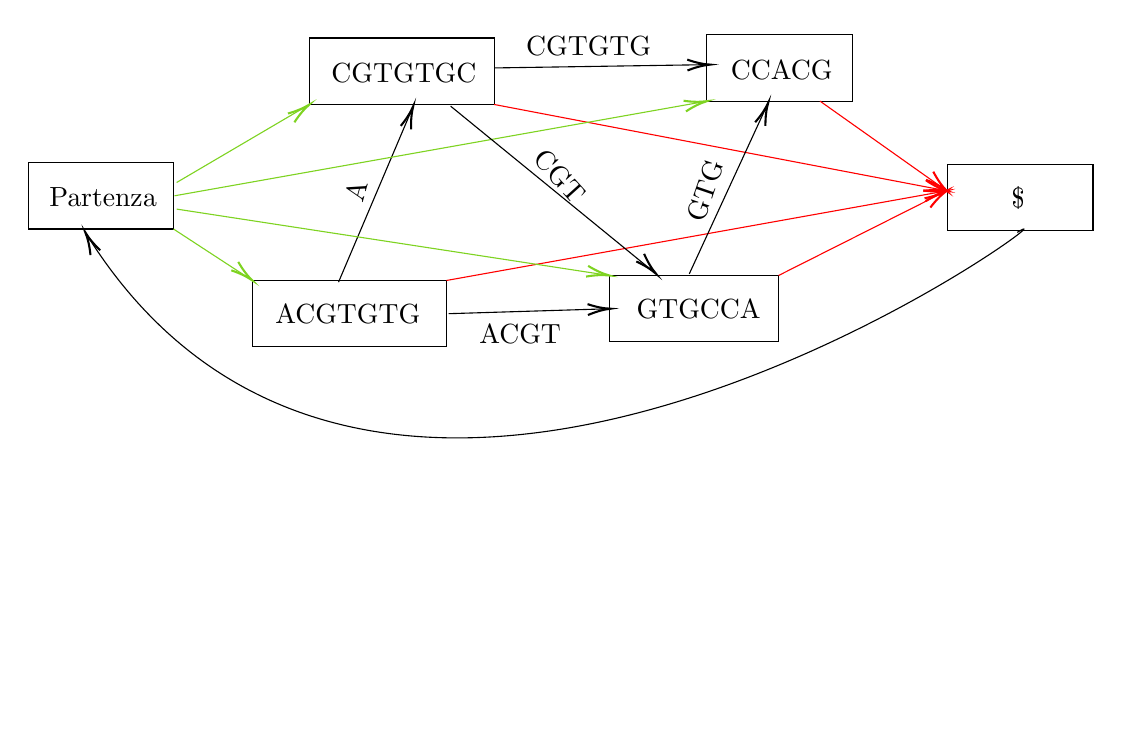
\begin{tikzpicture}[x=0.75pt,y=0.6pt,yscale=-1,xscale=1]
%uncomment if require: \path (0,281); %set diagram left start at 0, and has height of 281
%Shape: Rectangle [id:dp6560992130069507] 
\draw   (158.5,30) -- (247.5,30) -- (247.5,70) -- (158.5,70) -- cycle ;
%Shape: Rectangle [id:dp8633094909301302] 
\draw   (350,28) -- (420,28) -- (420,68) -- (350,68) -- cycle ;
%Straight Lines [id:da17421981355945193] 
\draw    (247.5,48) -- (349.5,46.04) ;
\draw [shift={(351.5,46)}, rotate = 538.9] [color={rgb, 255:red, 0; green, 0; blue, 0 }  ][line width=0.75]    (10.93,-3.29) .. controls (6.95,-1.4) and (3.31,-0.3) .. (0,0) .. controls (3.31,0.3) and (6.95,1.4) .. (10.93,3.29)   ;

%Shape: Rectangle [id:dp26552417711503384] 
\draw   (131,176) -- (224.5,176) -- (224.5,216) -- (131,216) -- cycle ;
%Shape: Rectangle [id:dp10524493499981546] 
\draw   (303,173) -- (384.5,173) -- (384.5,213) -- (303,213) -- cycle ;
%Straight Lines [id:da8474295750375322] 
\draw    (172.5,177) -- (207.86,72.89) ;
\draw [shift={(208.5,71)}, rotate = 468.76] [color={rgb, 255:red, 0; green, 0; blue, 0 }  ][line width=0.75]    (10.93,-3.29) .. controls (6.95,-1.4) and (3.31,-0.3) .. (0,0) .. controls (3.31,0.3) and (6.95,1.4) .. (10.93,3.29)   ;

%Straight Lines [id:da7595524463463148] 
\draw    (225.5,196) -- (301.5,193.08) ;
\draw [shift={(303.5,193)}, rotate = 537.8] [color={rgb, 255:red, 0; green, 0; blue, 0 }  ][line width=0.75]    (10.93,-3.29) .. controls (6.95,-1.4) and (3.31,-0.3) .. (0,0) .. controls (3.31,0.3) and (6.95,1.4) .. (10.93,3.29)   ;

%Shape: Rectangle [id:dp375619585347468] 
\draw   (466,106) -- (536,106) -- (536,146) -- (466,146) -- cycle ;
%Straight Lines [id:da8048124855752778] 
\draw [color={rgb, 255:red, 255; green, 0; blue, 0 }  ,draw opacity=1 ]   (404.5,68) -- (464,120.67) ;
\draw [shift={(465.5,122)}, rotate = 221.52] [color={rgb, 255:red, 255; green, 0; blue, 0 }  ,draw opacity=1 ][line width=0.75]    (10.93,-3.29) .. controls (6.95,-1.4) and (3.31,-0.3) .. (0,0) .. controls (3.31,0.3) and (6.95,1.4) .. (10.93,3.29)   ;

%Straight Lines [id:da91205814003782] 
\draw [color={rgb, 255:red, 255; green, 0; blue, 0 }  ,draw opacity=1 ]   (384.5,173) -- (463.81,123.07) ;
\draw [shift={(465.5,122)}, rotate = 507.8] [color={rgb, 255:red, 255; green, 0; blue, 0 }  ,draw opacity=1 ][line width=0.75]    (10.93,-3.29) .. controls (6.95,-1.4) and (3.31,-0.3) .. (0,0) .. controls (3.31,0.3) and (6.95,1.4) .. (10.93,3.29)   ;

%Straight Lines [id:da9132525115334023] 
\draw [color={rgb, 255:red, 255; green, 0; blue, 0 }  ,draw opacity=1 ]   (224.5,176) -- (463.55,122.44) ;
\draw [shift={(465.5,122)}, rotate = 527.37] [color={rgb, 255:red, 255; green, 0; blue, 0 }  ,draw opacity=1 ][line width=0.75]    (10.93,-3.29) .. controls (6.95,-1.4) and (3.31,-0.3) .. (0,0) .. controls (3.31,0.3) and (6.95,1.4) .. (10.93,3.29)   ;

%Straight Lines [id:da7445332124936079] 
\draw [color={rgb, 255:red, 255; green, 0; blue, 0 }  ,draw opacity=1 ]   (247.5,70) -- (463.55,121.54) ;
\draw [shift={(465.5,122)}, rotate = 193.42] [color={rgb, 255:red, 255; green, 0; blue, 0 }  ,draw opacity=1 ][line width=0.75]    (10.93,-3.29) .. controls (6.95,-1.4) and (3.31,-0.3) .. (0,0) .. controls (3.31,0.3) and (6.95,1.4) .. (10.93,3.29)   ;

%Curve Lines [id:da5406375819342921] 
\draw    (499.5,147) .. controls (539.5,117) and (195.5,440) .. (50.5,147) ;
\draw [shift={(50.5,147)}, rotate = 423.66999999999996] [color={rgb, 255:red, 0; green, 0; blue, 0 }  ][line width=0.75]    (10.93,-3.29) .. controls (6.95,-1.4) and (3.31,-0.3) .. (0,0) .. controls (3.31,0.3) and (6.95,1.4) .. (10.93,3.29)   ;

%Shape: Rectangle [id:dp7097560349466829] 
\draw   (23,105) -- (93,105) -- (93,145) -- (23,145) -- cycle ;
%Straight Lines [id:da08262697801168883] 
\draw [color={rgb, 255:red, 126; green, 211; blue, 33 }  ,draw opacity=1 ]   (94.5,117) -- (156.89,71.18) ;
\draw [shift={(158.5,70)}, rotate = 503.71] [color={rgb, 255:red, 126; green, 211; blue, 33 }  ,draw opacity=1 ][line width=0.75]    (10.93,-3.29) .. controls (6.95,-1.4) and (3.31,-0.3) .. (0,0) .. controls (3.31,0.3) and (6.95,1.4) .. (10.93,3.29)   ;

%Straight Lines [id:da5925934520006846] 
\draw [color={rgb, 255:red, 126; green, 211; blue, 33 }  ,draw opacity=1 ]   (93.5,125) -- (348.05,68.43) ;
\draw [shift={(350,68)}, rotate = 527.47] [color={rgb, 255:red, 126; green, 211; blue, 33 }  ,draw opacity=1 ][line width=0.75]    (10.93,-3.29) .. controls (6.95,-1.4) and (3.31,-0.3) .. (0,0) .. controls (3.31,0.3) and (6.95,1.4) .. (10.93,3.29)   ;

%Straight Lines [id:da9161535456154222] 
\draw [color={rgb, 255:red, 126; green, 211; blue, 33 }  ,draw opacity=1 ]   (94.5,133) -- (301.04,172.62) ;
\draw [shift={(303,173)}, rotate = 190.86] [color={rgb, 255:red, 126; green, 211; blue, 33 }  ,draw opacity=1 ][line width=0.75]    (10.93,-3.29) .. controls (6.95,-1.4) and (3.31,-0.3) .. (0,0) .. controls (3.31,0.3) and (6.95,1.4) .. (10.93,3.29)   ;

%Straight Lines [id:da5498196959860426] 
\draw [color={rgb, 255:red, 126; green, 211; blue, 33 }  ,draw opacity=1 ]   (93,145) -- (129.45,174.74) ;
\draw [shift={(131,176)}, rotate = 219.21] [color={rgb, 255:red, 126; green, 211; blue, 33 }  ,draw opacity=1 ][line width=0.75]    (10.93,-3.29) .. controls (6.95,-1.4) and (3.31,-0.3) .. (0,0) .. controls (3.31,0.3) and (6.95,1.4) .. (10.93,3.29)   ;

%Straight Lines [id:da4597957524218963] 
\draw    (226.5,71) -- (324.1,170.57) ;
\draw [shift={(325.5,172)}, rotate = 225.57] [color={rgb, 255:red, 0; green, 0; blue, 0 }  ][line width=0.75]    (10.93,-3.29) .. controls (6.95,-1.4) and (3.31,-0.3) .. (0,0) .. controls (3.31,0.3) and (6.95,1.4) .. (10.93,3.29)   ;

%Straight Lines [id:da11466253953137451] 
\draw    (341.5,172) -- (378.81,70.88) ;
\draw [shift={(379.5,69)}, rotate = 470.25] [color={rgb, 255:red, 0; green, 0; blue, 0 }  ][line width=0.75]    (10.93,-3.29) .. controls (6.95,-1.4) and (3.31,-0.3) .. (0,0) .. controls (3.31,0.3) and (6.95,1.4) .. (10.93,3.29)   ;


% Text Node
\draw (204,51) node  [align=left] {CGTGTGC};
% Text Node
\draw (386,49) node  [align=left] {CCACG};
% Text Node
\draw (177,196) node  [align=left] {ACGTGTG};
% Text Node
\draw (346,193) node  [align=left] {GTGCCA};
% Text Node
\draw (500,126) node  [align=left] {\$};
% Text Node
\draw (59,126) node  [align=left] {Partenza};
% Text Node
\draw (181,122) node [rotate=-285.42] [align=left] {A};
% Text Node
\draw (349,122) node [rotate=-288.92] [align=left] {GTG};
% Text Node
\draw (293,35) node  [align=left] {CGTGTG};
% Text Node
\draw (260,208) node  [align=left] {ACGT};
% Text Node
\draw (279,113) node [rotate=-47.91] [align=left] {CGT};
\end{tikzpicture}
\end{center}
\end{figure}

\subsection{TSP}
Un problema intermedio tra la visita nei grafi e la ricostruzione di stringhe è il Traveling Salesman Problem: dato un grafo orientato $G = \langle V, A \rangle$ con archi pesati $w : A \rightarrow \mathbb{Q}^+$, trovare una permutazione $\Pi = \langle \pi_1,\ \dots,\ \pi_n \rangle$ di $V$ di costo minimo che visiti tutti i nodi e torni al punto di partenza. Il costo è il peso totale di tutti gli archi attraversati.

La funzione obiettivo è:
\begin{equation*}
w(\pi_n, \pi_1) + \sum_{i=1}^{n} w(\pi_i, \pi_{i+1})
\end{equation*}

Nonostante sia risolvibile in pratica con grafi anche di grandi dimensioni (grazie alla potenza dell'hardware), il problema è NP-completo. 

Partendo dall'istanza della superstringa, si vuole ottenere un'istanza di TSP per poi arrivare alla relativa soluzione. Una volta trovata la soluzione TSP, essa viene convertita in quella della superstringa.

Le stringhe in ingresso vengono mappate nel grafo di TSP, diventando nodi. Gli archi devono avere peso minimo, quindi diventano la parte della stringa che non è sovrapposta. \\
Ogni read è una città, ma l'assemblaggio non è un ciclo e la lunghezza della stringa è diversa dal costo del percorso TSP. 

Si ha che:
\begin{equation*}
\abs{S} = \sum_{i=1}^{n} |s_i| - \sum_{i=1}^{n-1} |ov(s_i, s_{i+1})|
\end{equation*}
dove $ov$ è l'overlap.

Per individuare la fine della stringa si usa un simbolo di appoggio \$, collegato all'inizio, per poter tornare al punto di partenza. Vengono mappati tutti i possibili cammini, e poi viene individuato il percorso ottimo.

\subsection{OLC}
OLC (Overlap, Layout, Consensus) è un modo di eseguire la riduzione tramite questi passaggi:
\begin{enumerate}
	\item Overlap, calcolo delle sovrapposizioni e costruzione del grafo. Per un metodo esatto si utilizza il suffix array, altrimenti la programmazione dinamica;
	\item Layout, fusione dei cammini per ottenere i \textit{contigs}, sottosequenze continue. Le ripetizioni (branching nodes) vengono rimosse;
	\item Consensus, calcolo dei nucleotidi.
\end{enumerate}

Si vuole calcolare la lunghezza dell'overlap per ogni coppia di stringhe in modo veloce, usando i suffix array. Il primo step è calcolare il suffix tree generalizzato di tutte le read, e con una sola visita determinare per ogni prefisso se esso sia anche un suffisso.

L'albero viene visitato carattere per carattere, usando la read come pattern, e cercando tutti i nodi da cui esce un simbolo di terminazione che non sia l'ultimo. 

\subsubsection{OLC con errori}
Per avere overlap permettendo la presenza di errori, al contrario, si definisce un problema tale che: date due stringhe $s$, $t$, trovare:
\begin{enumerate}
	\item Suffisso $x$ di $s$;
	\item Suffisso $y$ di $t$;
\end{enumerate}
tale che $\abs{x} + \abs{y} - 2edit(x, y)$ sia massima. Il 2 viene introdotto arbitrariamente come fattore moltiplicativo per dare un peso maggiore alle sovrapposizioni.

In questo caso non vengono confrontati prefissi, ma un prefisso e un suffisso. $M[i, j] =$ ottimo del prefisso lungo $j$ di $t$ e del suffisso lungo $i$ di $s$. L'algoritmo è simile a LCS, con questa differenza. 

\subsection{SBH}
SBH, Sequencing By Hybridation, è una vecchia tecnologia (metà anni '90) per gli array di DNA, che analizza gli oligonucleotidi (6-10 basi). Per ogni $k$-mero (chip), con $k \sim 8$, si conosce se appare nel genoma. Il processo è chiamato DNA chip perché la logica di fondo è la stessa che viene usata per i chip, ognuno di essi può tenere migliaia di oligonucleotidi.

\begin{example}{}{}
	\begin{tabular}{l | *{13}{c}}
		DNA Chip		& A & C & G & T & G & G & C & A \\
		DNA Replicato	& T & G & G & \textbf{T} & \textbf{G} & \textbf{C} & \textbf{A} & \textbf{C} & \textbf{C} & \textbf{G} & \textbf{T} & G & G
	\end{tabular}
\end{example}

Ogni nucleotide viene messo in contatto con il DNA dopo che esso è stato replicato più volte tramite PCR (un processo chimico), nel quale avviene un'ibridazione: nelle giuste condizioni biochimiche, il nucleotide sul chip forma legami covalenti con una porzione di DNA che è perfettamente complementare (eliche), in modo che essi siano ancora uniti al momento dell'estrazione. 

Alcuni oligonucleotidi non reagiranno, perché non hanno trovato il proprio complementare: è possibile individuarli sapendo che il DNA replicato viene marcato con qualche sostanza che lo renda riconoscibile (fluorescente). 

Questa tecnologia in pratica non viene utilizzata, ma ha degli interessanti aspetti algoritmici. Una differenza essenziale tra un grafo di overlap e SBH è che i $k$-meri hanno tutti la stessa lunghezza, al contrario delle read, e ci si aspettano sovrapposizioni lunghe esattamente $k - 1$.

\subsubsection{Grafi di De Bruijn}
Ogni $k$-mero (sottostringa di lunghezza $k$) viene diviso in $(k - 1)$-meri: in un grafo di De Bruijn, ogni \textbf{arco} corrisponde a un $k$-mero, ogni \textbf{vertice} corrisponde a un $(k - 1)$-mero, e due vertici sono collegati se ci sono sovrapposizioni. 

Dato che tutte le stringhe in ingresso hanno lunghezza $k$ e sono presenti in almeno una read, il problema della costruzione del grafo diventa più semplice.

I $(k - 1)$-meri identici vengono eliminati, in modo da avere nodi distinti. Il problema diventa trovare in un grafo il \textit{percorso che attraversi ogni arco esattamente una volta} (cammino Euleriano), per ricostruire il genoma. 



\tikzset{every picture/.style={line width=0.75pt}} %set default line width to 0.75pt        

\begin{figure}[H]
\caption{Grafo di De Brujin}
\begin{center}
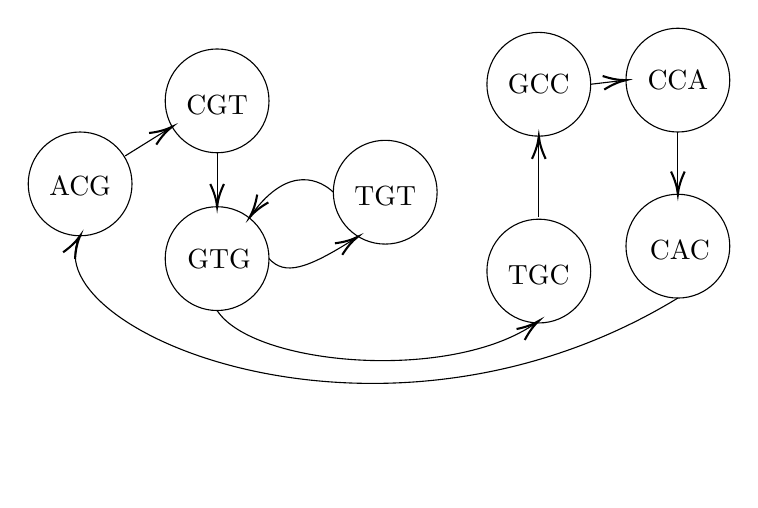
\begin{tikzpicture}[x=0.75pt,y=0.75pt,yscale=-1,xscale=1]
%uncomment if require: \path (0,248); %set diagram left start at 0, and has height of 248

%Shape: Circle [id:dp5662414203096264] 
\draw   (81,53) .. controls (81,39.19) and (92.19,28) .. (106,28) .. controls (119.81,28) and (131,39.19) .. (131,53) .. controls (131,66.81) and (119.81,78) .. (106,78) .. controls (92.19,78) and (81,66.81) .. (81,53) -- cycle ;
%Shape: Circle [id:dp13985089677551477] 
\draw   (81,129) .. controls (81,115.19) and (92.19,104) .. (106,104) .. controls (119.81,104) and (131,115.19) .. (131,129) .. controls (131,142.81) and (119.81,154) .. (106,154) .. controls (92.19,154) and (81,142.81) .. (81,129) -- cycle ;
%Shape: Circle [id:dp3574816316500795] 
\draw   (15,93) .. controls (15,79.19) and (26.19,68) .. (40,68) .. controls (53.81,68) and (65,79.19) .. (65,93) .. controls (65,106.81) and (53.81,118) .. (40,118) .. controls (26.19,118) and (15,106.81) .. (15,93) -- cycle ;
%Shape: Circle [id:dp6367614117013465] 
\draw   (162,97) .. controls (162,83.19) and (173.19,72) .. (187,72) .. controls (200.81,72) and (212,83.19) .. (212,97) .. controls (212,110.81) and (200.81,122) .. (187,122) .. controls (173.19,122) and (162,110.81) .. (162,97) -- cycle ;
%Shape: Circle [id:dp8286860889666687] 
\draw   (236,135) .. controls (236,121.19) and (247.19,110) .. (261,110) .. controls (274.81,110) and (286,121.19) .. (286,135) .. controls (286,148.81) and (274.81,160) .. (261,160) .. controls (247.19,160) and (236,148.81) .. (236,135) -- cycle ;
%Shape: Circle [id:dp04605576669499256] 
\draw   (236,45) .. controls (236,31.19) and (247.19,20) .. (261,20) .. controls (274.81,20) and (286,31.19) .. (286,45) .. controls (286,58.81) and (274.81,70) .. (261,70) .. controls (247.19,70) and (236,58.81) .. (236,45) -- cycle ;
%Shape: Circle [id:dp9155218336299027] 
\draw   (303,43) .. controls (303,29.19) and (314.19,18) .. (328,18) .. controls (341.81,18) and (353,29.19) .. (353,43) .. controls (353,56.81) and (341.81,68) .. (328,68) .. controls (314.19,68) and (303,56.81) .. (303,43) -- cycle ;
%Shape: Circle [id:dp766738912437283] 
\draw   (303,123) .. controls (303,109.19) and (314.19,98) .. (328,98) .. controls (341.81,98) and (353,109.19) .. (353,123) .. controls (353,136.81) and (341.81,148) .. (328,148) .. controls (314.19,148) and (303,136.81) .. (303,123) -- cycle ;
%Straight Lines [id:da9646625679785032] 
\draw    (61.75,79.5) -- (82.55,66.56) ;
\draw [shift={(84.25,65.5)}, rotate = 508.11] [color={rgb, 255:red, 0; green, 0; blue, 0 }  ][line width=0.75]    (10.93,-3.29) .. controls (6.95,-1.4) and (3.31,-0.3) .. (0,0) .. controls (3.31,0.3) and (6.95,1.4) .. (10.93,3.29)   ;

%Straight Lines [id:da8830983152823235] 
\draw    (106,78) -- (106,102) ;
\draw [shift={(106,104)}, rotate = 270] [color={rgb, 255:red, 0; green, 0; blue, 0 }  ][line width=0.75]    (10.93,-3.29) .. controls (6.95,-1.4) and (3.31,-0.3) .. (0,0) .. controls (3.31,0.3) and (6.95,1.4) .. (10.93,3.29)   ;

%Curve Lines [id:da7743744950450349] 
\draw    (131,129) .. controls (138.6,137.33) and (149.07,134.14) .. (172.31,119.42) ;
\draw [shift={(173.75,118.5)}, rotate = 507.41] [color={rgb, 255:red, 0; green, 0; blue, 0 }  ][line width=0.75]    (10.93,-3.29) .. controls (6.95,-1.4) and (3.31,-0.3) .. (0,0) .. controls (3.31,0.3) and (6.95,1.4) .. (10.93,3.29)   ;

%Curve Lines [id:da701157029011428] 
\draw    (162,97) .. controls (156.37,91.61) and (140.89,82.86) .. (122.86,107.45) ;
\draw [shift={(121.75,109)}, rotate = 304.92] [color={rgb, 255:red, 0; green, 0; blue, 0 }  ][line width=0.75]    (10.93,-3.29) .. controls (6.95,-1.4) and (3.31,-0.3) .. (0,0) .. controls (3.31,0.3) and (6.95,1.4) .. (10.93,3.29)   ;

%Curve Lines [id:da9534415928320956] 
\draw    (328,148) .. controls (184.94,235.12) and (18.86,163.46) .. (39.32,119.33) ;
\draw [shift={(40,118)}, rotate = 479.11] [color={rgb, 255:red, 0; green, 0; blue, 0 }  ][line width=0.75]    (10.93,-3.29) .. controls (6.95,-1.4) and (3.31,-0.3) .. (0,0) .. controls (3.31,0.3) and (6.95,1.4) .. (10.93,3.29)   ;

%Curve Lines [id:da9799576589537213] 
\draw    (106,154) .. controls (123.33,180.73) and (219.06,188.84) .. (259.78,159.89) ;
\draw [shift={(261,159)}, rotate = 503.13] [color={rgb, 255:red, 0; green, 0; blue, 0 }  ][line width=0.75]    (10.93,-3.29) .. controls (6.95,-1.4) and (3.31,-0.3) .. (0,0) .. controls (3.31,0.3) and (6.95,1.4) .. (10.93,3.29)   ;

%Straight Lines [id:da2213126680718589] 
\draw    (261,109) -- (261,72) ;
\draw [shift={(261,70)}, rotate = 450] [color={rgb, 255:red, 0; green, 0; blue, 0 }  ][line width=0.75]    (10.93,-3.29) .. controls (6.95,-1.4) and (3.31,-0.3) .. (0,0) .. controls (3.31,0.3) and (6.95,1.4) .. (10.93,3.29)   ;

%Straight Lines [id:da05405134063421202] 
\draw    (328,96) -- (328,68) ;

\draw [shift={(328,98)}, rotate = 270] [color={rgb, 255:red, 0; green, 0; blue, 0 }  ][line width=0.75]    (10.93,-3.29) .. controls (6.95,-1.4) and (3.31,-0.3) .. (0,0) .. controls (3.31,0.3) and (6.95,1.4) .. (10.93,3.29)   ;
%Straight Lines [id:da7142573004014958] 
\draw    (286,45) -- (301.01,43.23) ;
\draw [shift={(303,43)}, rotate = 533.29] [color={rgb, 255:red, 0; green, 0; blue, 0 }  ][line width=0.75]    (10.93,-3.29) .. controls (6.95,-1.4) and (3.31,-0.3) .. (0,0) .. controls (3.31,0.3) and (6.95,1.4) .. (10.93,3.29)   ;


% Text Node
\draw (40,94) node  [align=left] {ACG};
% Text Node
\draw (106,55) node  [align=left] {CGT};
% Text Node
\draw (107,129) node  [align=left] {GTG};
% Text Node
\draw (187,99) node  [align=left] {TGT};
% Text Node
\draw (261,45) node  [align=left] {GCC};
% Text Node
\draw (328,43) node  [align=left] {CCA};
% Text Node
\draw (261,137) node  [align=left] {TGC};
% Text Node
\draw (329,125) node  [align=left] {CAC};


\end{tikzpicture}
\end{center}
\end{figure}

\subsection{Cicli e cammini di Eulero}
\begin{definition}{Grafo Semi-Euleriano}{}
	Sia $G = \langle V, A \rangle$ un grafo orientato. $G$ è semi-Euleriano se esistono due vertici $s, t$ tali che $N_G^- (s) = N_G^+(s) + 1, N_G^-(t) = N_G^+(v) - 1$, mentre per ogni altro vertice $w$, $N_G^-(w) = N_G^+(w)$.
	
	Ogni nodo ha lo stesso numero di archi entranti e uscenti, tranne per due nodi di cui uno ha un arco uscente in più e l'altro uno in meno.
\end{definition}

\begin{definition}{Grafo Euleriano}{}
	Sia $G = \langle V, A \rangle $ un grafo orientato. $G$ è Euleriano se $N_G^-(w) = N_G^+(w)$, per ogni vertice (stesso numero di archi entranti e uscenti).
	\tcblower
	Sia $G = \langle V, A \rangle$ un grafo Euleriano e sia $C$ un ciclo di $G$. Sia $G_1$ il grafo ottenuto da $G$ togliendo tutti gli archi di $C$. Allora $G_1$ è Euleriano.
\end{definition}

\begin{thm}{Grafo Euleriano}{}
	Un grafo connesso $G = \langle V, A \rangle$ ha un cammino Euleriano se e solo se $G$ è semi-Euleriano. $G$ ha un ciclo Euleriano se e solo se $G$ è Euleriano.
	\tcblower
	Sia $G = \langle V, A \rangle$ un semi-Euleriano e sia $P$ un cammino da $s$ a $t$. Sia $G_1$ il grafo ottenuto da $G$ togliendo tutti gli archi di $P$. Allora $G_1$ è Euleriano.
\end{thm}

\begin{definition}{Ciclo Euleriano e Hamiltoniano}{}
	Un ciclo (cammino) Euleriano è un assemblaggio in un grafo orientato e connesso che attraversa ogni \textbf{arco} esattamente una volta.
	\tcblower
	Un ciclo Hamiltoniano (caso particolare di TSP) è un cammino che attraversa ogni \textbf{vertice} esattamente una volta.
\end{definition}

Il primo problema è risolvibile con un algoritmo in tempo lineare, mentre il secondo è NP-completo. 

Un ciclo viene chiamato semplice se non tocca due volte lo stesso vertice: è possibile trovare cicli Euleriani in questi casi, ma non ci saranno cicli Hamiltoniani. 

L'algoritmo è in tempo lineare: ciò significa che per ogni arco si spende un tempo costante. Si parte dal primo vertice, e si prosegue verso un arco uscente $s$. Si cercano sempre archi uscenti che non sono già stati visitati, e si termina quando non ne esistono più.

L'ultimo vertice è la destinazione, che ha un numero di archi entranti superiore di 1 rispetto agli archi uscenti. Togliendo il cammino Euleriano, il grafo diventa sicuramente Euleriano (formato da un insieme di cicli), anche se non necessariamente connesso. 

Ci dev'essere un vertice toccato dal cammino Euleriano che ha un arco uscente non ancora visitato. Come prima, si guarda quest'ultimo arco del vertice, e la procedura termina nello stesso di partenza: si è trovato un altro ciclo. 

I vari cicli, dopo essere stati trovati, vengono ricombinati.

\subsection{Reverse and complement}
All'algoritmo precedente viene aggiunta una complicazione: non si conosce lo strand di DNA. La stessa stringa potrebbe aver subito un reverse and complement, e non si sa quale delle due possibilità è effettivamente quella corretta.

Per evitare il raddoppio dello spazio di memoria, si indica la read canonica come la prima in ordine lessicografico, però a ogni calcolo dell'overlap viene considerato anche il complemento.

L'idea di base è che i valori più lunghi di $k$ sono più espressivi, perché permettono di gestire meglio le sovrapposizioni. I numeri dispari sono migliori, perché altrimenti potrebbero esistere $k$-meri che hanno reverse and complement uguali all'originale. 

Il genoma è diploide (copie quasi perfettamente identiche), ma le differenze formano percorsi separati in un grafo chiamato \textit{bolla} (\textbf{bubble popping}). La lunghezza dei percorsi è variabile, e alcuni di essi non portano da nessuna parte: vengono rimossi in un processo chiamato \textbf{tip removal}. Attraverso questo perfezionamento delle sequenze sono costruiti i contig.

Un'altra fase importante è, dato un frammento del DNA di origine, capire se ci sono match tra contigs per poterli inserire in porzioni adiacenti (perché sono diploidi). Non sono ancora conosciuti tutti i possibili match.
\section{DCT wavelets}
L'obiettivo dell'analisi è la riduzione delle ridondanze, spostandosi in uno spazio dove le informazioni e i canali sono separati. 

Nel dominio diretto le componenti di un segnale $X$ sono tra loro significativamente correlate, quindi la stessa informazione è ridondante. Spostandosi nel dominio trasformato $Y = T[X]$, si cerca una rappresentazione dove le componenti siano molto meno correlate.

$Y$ può essere codificato in modo più efficiente di $X$, utilizzando solo le componenti del segnale che descrivono l'informazione. Lo spettro, per esempio, ha un contributo maggiore espresso con le basse frequenze al centro, quindi è possibile codificare solo una porzione determinata di energia.

In termini di compressione, sono necessari solo i bit delle componenti da tenere. Il modello di compressione permette di quantizzare con perdite trascurabili, in un cambio di spazio secondo due strategie:
\begin{itemize}
	\item Codificatore di sorgente, che riduce le ridondanze;
	\item Codificatore di canale, che incrementa l'immunità al rumore.
\end{itemize}

\subsection{Codifica con trasformate}
Questo algoritmo introduce perdita ed è computazionalmente costoso, a causa del calcolo delle trasformate. Una trasformata lineare e reversibile è usata per il mapping dell'immagine in un set di coefficienti che vengono poi quantificati e codificati.

Il mapping può essere effettuato secondo diverse metodologie, a seconda della capacità di decorrelazione dei dati, semplicità di realizzazione e altri fattori.

La KLT (analisi alle componenti principali) è la trasformata ottima, ma è computazionalmente inefficiente. DCT, invece, approssima il comportamento ottimo, ed è usata negli algoritmi di codifica più utilizzati (jpeg, mpeg).

La trasformata wavelet permette la multirisoluzione (jpeg2000), e funziona secondo il principio di determinazione di Heisenberg, trovando un compromesso tra le frequenze e il dominio temporale lavorando con tradeoff.

Data una funzione $f(x)$, la sua DFT $F(u)$ è:
$$F(u) = \frac{1}{M} \sum_{x=0}^{M- 1}f(x)e^{-j\frac{2\pi}{M}ux} = \frac{1}{M} \sum_{x=0}^{M- 1}f(x)g(u, x)$$
$$g(u, x) = e^{-j\frac{2\pi}{M}ux}$$

La trasformata è lineare e invertibile, e $g(u, x)$ è detto kernel della trasformazione diretta, da cui dipendono le proprietà. I kernel devono essere invertibili, lineari e separabili.

Trasformata di Fourier discreta 1D:
$$e^{-j\frac{2\pi}{M}ux} = \cos\big(\frac{2\pi}{M}ux\big) + j\sin\big(\frac{2\pi}{M}ux\big)$$
% immagine onde quadrate
Il segnale di partenza è proiettato in base al suo tempo e spazio con le sue parti reale e immaginaria. Seno e coseno hanno simmetria rispettivamente dispari e pari, e trasformando si osserva l'influenza di ciascuna componente. 

La trasformata coseno discreta (DCT) è lineare, con kernel diretto uguale a quello inverso (simmetria speculare), separabile e simmetrico. La componente continua è legata al valore medio dell'immagine (0, 0). 
$$T(u) = \sum_{x=0}^{M- 1}f(x)g(u, x) \qquad g(x, u) = \alpha(u) \cos\Big[\frac{(2x + 1)\pi u}{2N}\Big]$$
% immagine coseno
$$\alpha(u) = \begin{cases}
\sqrt{\frac{1}{N}} & u = 0 \\
\sqrt{\frac{2}{N}} & u = 1, 2, \dots, N - 1^{}
\end{cases}$$

La separabilità permette di calcolare la trasformata 2D tramite applicazioni successive della trasformata 1D alle righe e alle colonne, senza perdita di informazione. Ciascun blocco è costituito da $N \times N$ sottoblocchi.

Una maggiore quantità di informazione è presente nei primi coefficienti della DCT, rispetto allo stesso numero di coefficienti della DFT.
% dct vs dtf
Visualizzando un'immagine su un monitor con un range elevato (scala logaritmica), non si vede nulla perché il monitor arriva solo fino a 256.

\subsection{Analisi multirisoluzione}
Le immagini sono generalmente costituite da regioni connesse che formano gli oggetti, omogenee rispetto a una qualche proprietà.

L'analisi multirisoluzione permette di mettere in evidenza sia le immagini a bassa frequenza che quelle ad alta, con segnali e campioni di dimensioni diverse, concentrandosi su differenti posizioni nello spettro. 

Le caratteristiche locali di un'immagine sono contraddistinte da variazioni statistiche locali, dovute  discontinuità fra regioni omogenee. Caratteristiche nascoste a una data risoluzione possono essere individuabili a un'altra.

La tecnica più frequente è l'analisi piramidale, che parte dalla risoluzione massima e progressivamente sottocampiona, evidenziando i cambiamenti tra i dettagli e le perdite tra un livello e l'altro ricostruendo ogni volta l'immagine con meno dettagli. I pixel mancanti vengono approssimati tramite wavelet.

Il segnale è decomposto in un insieme di sottosegnali (sottobanda, analisi), passando attraverso filtri complementari, ciascuno dei quali agisce su una fascia di frequenze. Ricampionando, filtrando e ricombinando le sottobande (sintesi) si ottiene un'approssimazione $\hat{x}(n)$ dell'originale, non incorrendo in aliasing. 

Ciascuna sottobanda $(y_0(n), y_1(n))$ è ottenuta filtrando con un passa-banda $(h_0(n), h_1(n))$ il segnale originale. Poiché la sottobanda ha spettro limitato e pari a metà dell'originale, è possibile sottocampionare senza perdita di informazione. 
% immagine
%% da qui
Imponendo ..., si trovano le coppie di filtri di sintesi e corrispondenti filtri di analisi che garantiscono una perfetta ricostruzione. In caso di più dimensioni, possono esserci $n$ filtri per righe e colonne che mettono in evidenza diverse porzioni di frequenze rispetto alla direzione. 

Dato che le statistiche locali sono facilmente modellabili e presentano molti valori nulli, questa codifica è particolarmente vantaggiosa per la compressione: non tutto l'istogramma viene occupato, oppure ci sono poche alte frequenze che possono essere eliminato. L'approccio di denoising per ridurre il rumore è utilizzato nelle applicazioni mediche.

Il filtro passa-basso è una funzione di scala, mentre il passa-alto è una wavelet generata a partire da una wavelet madre. La formula in notazione monodimensionale è:
$$f(x)  = \frac{1}{den\sqrt{m}} \sum_{k} W_\varphi (j_0, k) \varphi_{j_0, k} (x) + \frac{1}{den\sqrt{m}} \sum_{j=j_0}^{J}\sum_{k} W... $$
Trasformando con la wavelet, è possibile pesare ogni contributo per capire quali frequenze e bande hanno influenza maggiore, valutando le features che caratterizzano l'immagine. 

Per calcolare gli edge, si ha il segnale di partenza in una somma di contributi: la parte interessata viene tenuta applicando la formula, mentre le altre componenti vengono annullate. 

Un altro approccio è il denoising, a partire dalle wavelet. La ricostruzione è effettuata dopo aver posto una soglia alta sui coefficienti a tutte le risoluzioni, accettando solo i valori al di sopra. 

\section{Tecniche di compressione}
Le tecniche di compressione si dividono in due grandi famiglie: lossy (con perdita accettabile a seconda dell'applicazione) e lossless (senza perdita). I dati ridondanti vengono rimossi, e il risparmio viene misurato tramite un rapporto di compressione in bit, dipendente appunto dalla ridondanza. 

Un tipo di ridondanza è statistico: i vicini possono essere correlati o dipendenti, quindi una parte dell'informazione è ripetuta. Alcuni livelli secondo l'istogramma hanno una maggiore probabilità di essere occupati, quindi è possibile calcolare il numero medio normalizzato di bit necessari per ogni frequenza. 

\section{Tecniche di compressione}
Il costo di un segnale dipende da campionamento e quantizzazione, fino ad arrivare a una quantità troppo elevata di dati per la memorizzazione ad alta qualità.

Per rappresentare l'informazione si ricorre alla compressione, cioè la trasformazione in un insieme di dati statisticamente incorrelati che garantiscano un grado di fedeltà (qualità) rispetto all'originale, e abbiano un accettabile peso computazionale per il tipo di applicazione.

Le tecniche di compressione si dividono in due grandi famiglie: lossy (con perdita accettabile a seconda dell'applicazione) e lossless (senza perdita). I dati ridondanti vengono rimossi, e il risparmio viene misurato tramite un rapporto di compressione in bit, dipendente appunto dalla ridondanza. 

I dati sono gli strumenti tramite i quali è rappresentata l'informazione, e quest'ultima può essere associata a diversi quantitativi di dati. Il principio della compressione è appunto minimizzare il numero di bit utilizzati. 
$$\text{rapporto di compressione } C = \frac{b_1 \text{ bit prima della compressione}}{b_2 \text{ bit dopo la compressione}}$$
$$\text{ridondanza relativa } R = 1 - \frac{1}{C}$$
Se $b_1 = b_2$, allora $R = 0$ e non ci sono dati ridondanti tra le due rappresentazioni. Un rapporto tipico di compressione è $10 : 1$, con corrispondente ridondanza $0.9$.

\subsection{Ridondanza}
Possono essere individuati diversi tipi di ridondanza, di cui almeno uno va ridotto:
\begin{enumerate}
	\item Della codifica;
	\item Spaziale o temporale (correlazione inter-campione);
	\item Percettiva, imponendo quantizzazioni più o meno spinte.
\end{enumerate}

I primi due consistono nella ridondanza statistica: i vicini possono essere correlati o dipendenti, quindi una parte dell'informazione è ripetuta. 

\subsubsection{Ridondanza della codifica}
La ridondanza della codifica non introduce perdita, quindi è reversibile e ha una soglia massima di compressione che può essere raggiunta. Quest'ultima dipende dal tipo di segnale.

L'idea è costruire un quantizzatore che venga usato nel miglior modo possibile, distribuendo i valori in modo equiprobabile tra i livelli. Alcuni livelli, secondo l'istogramma a livelli di grigio, hanno una maggiore probabilità di essere occupati, quindi è possibile calcolare quanto comprimere in base al numero medio normalizzato di bit necessari per ogni frequenza.

Se i valori sono sbilanciati, si ricorre alla codifica a lunghezza variabile, con numero di bit medio necessario per descrivere l'immagine:
$$L_{avg} = \sum_{k=0}^{L-1}l(r_k)p_r(r_k)$$
$l(r_k)$ è il numero di bit necessario per descrivere il $k$-esimo livello $r$, con frequenza (probabilità) $p_r$. Essendo gli standard a 256 livelli di grigio, la frequenza sarà costante e la sommatoria sarà 1, pertanto le immagini saranno codificate a $M\times N \cdot 8$ bit.

VLC (Variable-Length Coding) è una strategia di riduzione della ridondanza che impiega un numero minor di bit per rappresentare i livelli più probabili, e viceversa. Il numero medio di bit è minore rispetto alla lunghezza fissa.

\subsubsection{Ridondanza spaziale}
Quando l'istogramma è uniforme, però, la VLC non ha effetto. Tutti i valori sono equiprobabili, ma ciò li rende fortemente correlati (e pertanto ridondanti) spazialmente. Questo succede per esempio in immagini a righe, mentre lungo le colonne i valori sono incorrelati.

Si può ridurre la ridondanza spaziale individuata introducendo coppie run-length: il primo componente della coppia individua l'intensità, mentre il secondo il numero di volte con cui si ripete. L'approccio è lossless.

\subsubsection{Ridondanza percettiva}
L'immagine è percepita come se avesse un valore di grigio uniforme, ma l'istogramma è discordante da questa rappresentazione.

\begin{figure}[h]
	\centering
	\includegraphics[scale=0.4]{Lezioni/Immagini/ridondanzapercettiva}
\end{figure}

Le informazioni ignorate dal sistema visivo umano possono essere eliminate, sostituite da un valore medio. Il processo è eseguito tramite quantizzazione, ma c'è perdita. 

\subsection{Entropia}
L'entropia è la misura della quantità di dati minima necessaria per codificare senza perdita una sorgente di informazione, modellando la sorgente come processo probabilistico con eventi statisticamente indipendenti.

Informalmente, rappresenta il valore dell'informazione attraverso incertezza e probabilità di un certo simbolo. La sorgente deve emettere valori tra di loro incorrelati, quindi non deve avere memoria. 

Nel caso delle immagini, c'è molto spesso dipendenza tra pixel contigui, ma l'entropia è la soluzione ottima a cui avvicinarsi il più possibile.

Un evento casuale $E$ con probabilità $p(E)$ ha un grado di incertezza (e una quantità di informazione) pari a:
$$I(E) = \log \frac{1}{p(E)}$$
La base del logaritmo dipende dall'unità di misura dell'informazione, in questo caso 2 (bit). Se un evento è certo, l'incertezza è nulla. 

Essendo l'entropia proporzionale all'incertezza, l'entropia di una sorgente con alfabeto $S = \{s_1, s_2, \dots,s_M\}$ è:
$$H(S) = \sum_{k=1}^{M} p_k \log_2 \frac{1}{p_k} = -\sum_{k=1}^{M}\log_2p_k$$
$p_k$ è la probabilità del $k$-esimo simbolo dell'alfabeto, e $\log_2\frac{1}{p_k}$ è la quantità di informazione contenuta nel simbolo $s_k$, cioè il numero di bit necessario per la codificaLa . situazione di equiprobabilità genera entropia massima.

L'entropia indica pertanto un limite inferiore (valore medio) per il numero di bit necessari per codificare un certo alfabeto, ipotizzando l'equiprobabilità di ogni livello e fornendo un punto di riferimento per i codici a lunghezza variabile. 

L'obiettivo di VLC è trovare il codice di lunghezza minima per descrivere il segnale. Se un codice $c_1, c_2, \dots, c_M$ ha parole con lunghezza $b_1, b_2, \dots, b_M$, il numero medio di bit richiesti è:
$$R = \sum_{k=1}^{M}b_kp_k$$
Il problema della progettazione di codice è la ricerca di parole con lunghezza media vicina all'entropia della sorgente del segnale, cioè $r$ vicino a $H$, e la stima della precisione dei valori di probabilità.

La massima entropia implica un contenuto informativo visivo basso, essendo i valori equiprobabili. Immagini diverse possono avere entropia simile, ma essa serve come valore di riferimento solo con sorgenti senza memoria, quindi il rapporto di compressione può essere molto differente in caso di fotografie o immagini con pattern.

\subsubsection{Codici di Huffman}
La codifica di Huffman funziona come VLC: ai caratteri più frequenti vengono assegnate parole di pochi bit, quindi la lunghezza è inversamente proporzionale alla probabilità.

La compressione è senza perdita, e i codici possono essere costrutiti con una struttura da albero binario, generando un codice ottimale minimizzando $L_{avg}$ in modo che sia il più vicino possibile all'entropia della sorgente.

Se il segnale viene letto sequenzialmente, non si hanno informazioni precise riguardo alla distribuzione dei simboli: essa viene stimata tramite strumenti che aggiornano a ogni valore la possibile frequenza.

\subsection{RLC}
La correlazione tra bit può portare a un elevato risparmio, ma per ottenerla si deve ricorrere a sorgenti con memoria e algoritmi come RLC  (Run-Length Coding). 

Se ci sono raggruppamenti, è possibile sfruttare la memoria codificando il simbolo con la lunghezza del corrispondente gruppo. Il segnale si presenta con tanti 0 in sequenza intervallati da 1, e viene trasmessa la coppia di valore assunto e numero di valori. 

Gran parte del contenuto informativo di un pixel è ridondante, e può essere ottenuto a partire dai pixel vicini passando a un mapping più efficiente, ma generalmente non interpretabile visivamente. 

RLC considera singolarmente le linee dell'immagine, collezionando le coppie $(g, w)$ che indicao rispettivamente il valore e la lunghezza.

Questa tecnica è impiegata per la codifica di immagini a colori, ma è poco efficiente per immagini reali a causa delle imprecisioni e del rumore. 

Il bitmap prevede una modalità di compressione senza perdita utilizzando appunto RLC, codificando le informazioni sequenziali ripetute. Il rapporto di compressione può essere minore di 1 in caso che nuovi bit vengano sprecati per creare coppie di valori diversi da quelli non contigui.

\subsection{Differential coding}
Questa tecnica viene applicata quando RLC è inefficiente, e ha come scopo la riduzione della ridondanza in simboli consecutivi di un datastream. Nel caso di audio, si utilizza la variante DPCM (Differential Pulse Code Modulation).

PCM (Pulse Code Modulation) converte forme d'onda analogiche in segnali digitali attraverso:
\begin{itemize}
	\item Campionamento;
	\item Quantizzazione;
	\item Codifica, in genere binaria.
\end{itemize}

Osservando il segnale in termine di differenza tra frequenze, una forte correlazione spaziale viene sfruttata tramite codifica a lunghezza variabile sui picchi dell'istogramma.

DCPM calcola la differenza tra frequenze adiacenti, ed essa viene codificata. Il segnale viene ricostruito sommando le differenze a partire dal valore iniziale (noto).

Nel caso delle immagini, si opera generando un'immagine differenza fra pixel contigui applicando un operatore che approssima la derivata prima (gradiente) o seconda (Laplaciana):
$$d(x, y) = I(x, y) - I(x - 1, y)$$
$$d(x, y) = 4I(x, y) - I(x, y - 1) - I(x, y + 1) - I(x + 1, y) - I(x - 1, y)$$
Per sfruttare la ridondanza tenendo conto delle differenze, è possibile anche sfruttare la differenza tra il valore attuale e quello predetto. Se la regione è uniforme in base a determinate regole, sarà immediato il calcolo del valore successivo, sfruttando l'interpolazione. 

La differenza, con valori accurati, tenderà a 0 con un istogramma stretto, e di conseguenza un'entropia minore (MPEG) in presenza di ridondanza spaziale. 

\subsection{Algoritmi lossless}
Lossless JPEG non usa la DCT e non introduce perdita utilizzando la codifica predittiva, sfruttando l'uniformità delle regioni. 

Valuta le differenze tra il valore effettivo del pixel $x$ e il suo valore predetto dai pixel adiacenti sopra e a sinistra. La sequenza di valori viene poi codificata con VLC, riportando il primo pixel identicamente. 

Gli algoritmi lossless universali non richiedono la conoscenza a priori della distribuzione di probabilità dei simboli: in genere riescono a modellare dinamicamente le caratteristiche dei dati, adeguando la codifica.

Alcuni esempi di algoritmi sono Adaptive Huffman Coding, Lempel-Ziv e Arithmetic Coding. In funzione di com'è costruita l'immagine, ciascun algoritmo sarà più o meno efficiente. 

\newpage
\subsubsection{LZW}
 \begin{wrapfigure}{R}{0.4\textwidth}
	\vspace{-15pt}
	\includegraphics[width=0.4\textwidth]{Lezioni/Immagini/dizionario}
	\vspace{-20pt}
\end{wrapfigure}

LZW rimuove ridondanza di codifica e spaziale senza necessità di conoscenza a priori della probabilità di occorrenza dei simboli.

Viene inizialmente costruito un dizionario che contiene i simboli da codificare, con un ulteriore bit che permette di identificare l'occorrenza dei valori. Tutte le volte che un valore si ripete, la codifica può essere riutilizzata usando la coppia e associandola a un livello (analisi delle frequenze). 

\subsection{Codifica video}
Nei video esiste una correlazione non solo tra i pixel dello stesso fotogramma, ma anche tra fotogrammi adiacenti. In base alla ridondanza, è possibile applicare:
\begin{itemize}
	\item Compressione spaziale, intra-frame applicata a ciascuna immagine;
	\item Compressione temporale, inter-frame.
\end{itemize}

La codifica predittiva rimuove entrambe le tipologie, con un errore di predizione $e(n)$ ottenuto tramite VLC e diversi modelli di predizione.

\begin{figure}[h]
	\centering
	\includegraphics[scale=0.5]{Lezioni/Immagini/codificapredittiva}
\end{figure}

\subsection{Ridondanza percettiva}
In presenza di un segnale sonoro a una generica frequenza, si ha un'alterazione della soglia di udibilità per le frequenze limitrofe al segnale, che non vengono percepite: non tutta l'informazione ha la stessa importanza. 

La riduzione di ridondanza percettiva comporta quantizzazione, quindi è irreversibile e lossy dato che tiene conto solo delle componenti effettivamente udibili.

Gli schemi di compressione percettivi comprimono il segnale eliminando la parte non percepita dall'orecchio umano. Il masking può essere delle frequenze o temporale: quest'ultimo è effettuato saturando il sistema uditivo in modo da alterare le condizioni uditive (rumori forti alternati da deboli).

La ridondanza psicovisuale è un fenomeno legato alla legge di Weber: la sensibilità alle variazioni di luminosità diminuisce con la diminuzione della luminosità (immagine scura). Questo permette una maggiore quantizzazione nelle zone più scure.

L'occhio umano è più sensibile al rumore nelle regioni a bassa frequenza (uniformi) piuttosto che ad alta, e alle variazioni di luminanza piuttosto che crominanza. 

La quantizzazione IGS permette di convertire l'errore di quantizzazione alle basse frequenze in rumore ad alte frequenze, meno percepibile. L'effetto è l'eliminazione dei falsi contorni (dithering). 

I canali cromatici possono essere compressi mantenendone l'intensità, per poi ricostruire in base a questa informazione. 

\section{Valutazione della qualità di compressione}
Un sistema per la compressione di immagini è generalmente formato da unità strutturali distinte:
\begin{itemize}
	\item Codificatore o compressore:
	\begin{itemize}
		\item Di sorgente, che riduce la ridondanza del segnale operando sulle ridondanze spaziali e temporali, percettive e di codifica;
		\item Di canale, che incrementa l'immunità al rumore;
	\end{itemize}
	\item Decodificatore, che svolge le operazioni inverse:
	\begin{itemize}
		\item Di sorgente;
		\item Di canale.
	\end{itemize}
\end{itemize}

Le tecniche lossless non consentono di raggiungere rapporti di compressione superiori a $10 : 1$, effettuando solo mapping e codifica di simbolo senza quantizzazione.

La qualità della compressione si valuta una volta introdotta la quantizzazione nella fase di codifica, perché è l'unico caso in cui viene introdotta perdita di dati non ripetuti. 

La perdita di informazione permette di raggiungere rapporti fino a $100 : 1$, cercando un compromesso tra accuratezza e dimensioni. La qualità deve essere misurata quantitativamente secondo criteri oggettivi, considerando la presenza di ridondanze. 

Alcuni criteri sono:
$$\text{Segnale errore: } e(x y) = \hat{f}(x, y) - f(x, y)$$
$$\text{Errore totale: } \sum_{x=0}^{M-1} \sum_{y=0}^{N-1} e(x, y) = \sum_{x=0}^{M-1} \sum_{y=0}^{N-1} \hat{f}(x, y) - f(x, y)$$
$$\text{Root Mean Square error: } e_{rms} = \bigg[ \frac{1}{MN} \sum_{x=0}^{M-1} \sum_{y=0}^{N-1} \big[\hat{f}(x, y) - f(x, y)\big]^2\bigg]^{\frac{1}{2}}$$
$$\text{Signal to Noise Ratio: } SNR = \frac{\sum_{x=0}^{M-1} \sum_{y=0}^{N-1} \hat{f}(x, y)^2}{\sum_{x=0}^{M-1} \sum_{y=0}^{N-1} \big[\hat{f}(x, y) - f(x, y)\big]^2}$$
Il segnale errore restituisce un'immagine. RMS, il più comune, serve a normalizzare l'errore totale, dato che sommare valori di segno opposto potrebbe risultare in un numero prossimo a 0. SNR è già adottato per la quantizzazione, ma non è modellabile: è definito come il rapporto tra il segnale originale e la differenza, da minimizzare.

Le metriche non tengono in considerazione la percezione soggettiva: un algoritmo può commettere errori specifici non individuabili dalle formule, ma soltanto dall'occhio umano: sono necessari test soggettivi con valutazioni della qualità su scala predefinita e correlata con valori oggettivi. A parità di errore, una diversa tecnica di compressione potrebbe essere migliore o peggiore. 

\subsection{Codifica con trasformate}
La codifica con trasformate è un algoritmo lossy utilizzato per la compressione JPEG, che opera nel dominio trasformato. 

Trasformata diretta e inversa:
$$T(u, v) =  \sum_{x=0}^{M-1} \sum_{y=0}^{N-1} f(x, y) g(x, y, u, v)$$
$$f(x, y) = \sum_{y=0}^{M-1} \sum_{v=0}^{N-1} T(u, v) h(x, y, u, v)$$

La codifica attraverso i coefficienti della trasformata prepara alle successive fasi di compressione, in cui i coefficienti con ampiezza poco significativa sono quantizzati.

Il valore medio viene sostituito ai pixel che vengono rimossi: nel caso 2$\times$2 ci sono 4 coefficienti che vengono sostituiti da un componente, ma all'aumento del numero la correlazione tra pixel adiacenti diminuisce fino a rendere impossibile la riduzione senza perdite significative.

Diverse tipologie di coppie di trasformata e antitrasformata impiegabili:
\begin{itemize}
	\item KLT, analisi alle componenti principali, decorrela i dati ma computazionalmente inefficiente;
	\item DCT, approssima meglio il comportamento ottimo; 
	\item DFT;
	\item \dots
\end{itemize}

Viene utilizzata la trasformata lineare reversibile coseno 8$\times$8 con eliminazione di una parte dei coefficienti in base all'ampiezza, perché è il metodo che assicura un errore minore approssimando meglio il segnale a parità di numero di coefficienti. 

La dimensione $n$ della sotto-immagine è una potenza di 2 per semplicità computazionale, e all'aumentare di $n$ viene persa efficienza fino a un massimo valore di 20. Per questo motivo si preferisce 8 a 16.

64 bit permettono di rappresentare un numero di colori sufficiente, e al crescere di $n$ diminuisce la correlazione tra i pixel.

\newpage
\subsection{Compressione wavelet}
I coefficienti della trasformata decorrelano il contenuto informativo dei pixel di un'immagine, permettendo una codifica più efficiente anche se con un maggior numero di operazione.

La maggior parte dell'informazione è contenuta in un numero limitato di coefficienti, e i restanti possono essere opportunamente quantizzati con scarsa influenza sulla distorsione.

Scelto il livello $J$ di analisi, la trasformata wavelet decompone l'immagine evidenziando i coefficienti legati alle caratteristiche di ogni dimensione, effettuando un'analisi statistica che evidenzia contenuto informativo legato alle basse frequenze.

Al crescere del rapporto di compressione, si ha una crescente perdita dei dettagli, in particolare texture ed edge, con conseguente smoothing, ma la qualità rispetto a DCT rimane superiore grazie all'assenza di blocchettizzazione.

Il numero di operazioni dipende dalla metodologia utilizzata (Haar, Daubechies, symlet, C-D-F) ed è  proporzionale all'efficienza. Un altro fattore importante è il numero di livelli della decomposizione wavelet, generalmente non superiore a 3.




\section{Algoritmi NP-completi}
Lo studio della NP-completezza formalizza il concetto di problemi risolvibili in tempo polinomiale, e le proprietà di chiusura del loro insieme.

Ci sono due questioni che vanno affrontate: l'esistenza di una soluzione in termini di algoritmo (problemi indecidibili), e i tempi di calcolo accettabili (problemi intrattabili, non risolvibili rapidamente).

In base alla complessità, i problemi vengono divisi in classe: una classe è quindi l'insieme di problemi che, se esiste una soluzione, possono essere risolti da una macchina $M$ usando $O(f(n))$ della risorsa $R$, con dimensione dell'input $n$.

Esempio di problema indecidibile: halting problem. \\
Esempio di problema intrattabile: qualsiasi algoritmo che richieda $2^n$. 

Un problema di decisione ha solo due possibili risposte: sì o no (al contrario dei problemi computazionali). Alcuni problemi di decisione sono NP-completi.

La classe P ha come istanze linguaggi, e si può descrivere come i problemi di decisioni prese in tempo polinomiale da una macchina di Turing. $P$ rappresenta la classe problemi risolti da $T_M$ in tempo $P(n)$, cioè $T_M(n) = O(P(n))$ dove $P(n)$ è un polinomio in $n$.

Le categorie di algoritmi, quindi, si dividono in:
\begin{itemize}
	\item Risolvibili in tempo polinomiale, rappresentati da P;
	\begin{itemize}
		\item Esempio: trovare un arco di peso minimo in un grafo;
	\end{itemize}
	\item NP, non deterministici, per le quali le istanze che rispondono in modo affermativo al problema di decisione possono essere verificate in tempo polinomiale;
	\begin{itemize}
		\item Esempio 1: esistenza di un cammino provando tutte le combinazioni. Questo non implica che non esista un algoritmo migliore, ma se non esiste va dimostrato (da qui $P \subseteq NP$);
		\item Esempio 2: i test di primalità, fino a qualche decennio fa era NP, ma ora ci sono modi per risolverlo in tempo polinomiale;
		\item Esempio 3: decifratura della crittografia;
	\end{itemize}
	\item NP-completi, sottoinsieme di NP con problemi che hanno tutte le stesse caratteristiche, in cui ogni problema è riducibile a tutti gli altri in tempo polinomiale:
	\begin{itemize}
		\item Se si risolve un singolo algoritmo NP-completo, si ha il modo per risolvere tutti gli altri;
		\item Se anche solo un NP non ha soluzione in tempo polinomiale, sicuramente nessun NP-completo avrà soluzione;
		\item Ogni problema NP-completo appartiene a NP, e può essere ridotto a P; 
		\begin{itemize}
			\item Esempio: Traveling Salesman Problem;
		\end{itemize}
	\end{itemize}
	\item NP-hard, che rappresenta i problemi NP-completi riducibili uno all'altro in tempo polinomiale;
	\begin{itemize}
		\item Sono i problemi che sono almeno difficili quanto gli NP-completi, non necessariamente di decisione;
		\item Tutti i problemi NP possono essere ridotti a NP-hard in tempo polinomiale.
	\end{itemize}
\end{itemize}

$P \subseteq NP$ è uno dei principali quesiti in ambito informatico, e consiste nel capire se per ogni problema la cui soluzione è verificata in tempo polinomiale, esiste anche un modo per risolverlo in tempo polinomiale. 

Un problema in P ha come limite superiore un tempo esponenziale, così come gli NP, ma esistono problemi al di fuori da questi insiemi che comunque hanno la stessa complessità computazionale: quest'ultima classe è definita \textbf{exp}.

\subsection{Macchine di Turing}
Per stabilire il tempo di computazione si utilizza una \textbf{funzione di complessità}: \\
$T_M(n) = max\{t_M(x)\ |\ |x| = n\}$, dove $T_M$ è una macchina di Turing.

NB: è importante ricordare che una $T_M$ può entrare in loop infinito. In generale, una macchina di Turing computa funzioni su stringhe oppure decide e accetta linguaggi, cioé risponde all'accettazione di un determinato input.

Alcuni algoritmi non hanno una collocazione precisa negli insiemi: non esiste un modo per risolverli in tempo polinomiale, ma non è stato dimostrato che serve un tempo esponenziale. 

I problemi in P vengono rappresentati con una macchina di Turing che può essere deterministica o non deterministica: la classe di linguaggi accettata e la potenza è la stessa.

Esempio di linguaggio con $T_M$ deterministica: $\{a^nb^n\}$, con il relativo problema di decisione. \\
Esempio di linguaggio con $T_M$ non deterministica: $\{a^nb^n\} \cup \{a^nb^{2n}\}$, in cui all'inizio c'è la scelta tra quale dei due insiemi contiene la stringa. 

Una $T_M$ non deterministica è più veloce, perché il suo tempo di calcolo è: \\
$t_n(x) = \{|B| \mid \text{B è ramo più breve accettante se } X \in L\ \lor\ \text{B è ramo più lungo rifiutante se } X \notin L\}$.


% todo hamilton






%\newpage
\section{Inversioni}

\subsection{Il problema}

Come si misura la somiglianza o differenza di gusti? \\
Un esempio banale è il seguente:
\begin{gather*}
    L_A = \{1, 2, 3, 4, 5\}\\
    L_B = \{2, 4, 1, 3, 5\}
\end{gather*} \\
$L_A, L_B$ rappresentano due liste di film ordinati(con gli stessi numeri) e numerati secondo le preferenze rispettivamente di $A$ e $B$. \\
La differenza deve essere $0$ se $L_B = L_A$, e crescere fino ad avere il valore massimo quando $L_B$ è completamente "rovesciata" rispetto ad $L_A$.

\subsection{Il modello}

Una misura naturale è \textbf{il numero di inversioni(o scambi) tra film che devo fare per ricostruire } $L_A$ \textbf{ da } $L_B$ \\
Più in generale, si può arrivare alla seguente definizione:

\begin{definition}[Inversione]
    Data una sequenza di numeri $a_1,a_2,\dots,a_n$, una inversione è una coppia di indici $i < j$ tale che $a_i > a_j$.
\end{definition} ~\\
Questa definizione ci dice praticamente quanti scambi bisogna effettuare affinché l'array risulti ordinato.
$$\begin{tikzpicture}
    \matrix (m) [matrix of math nodes, row sep=2em,
      column sep=1em]{
      L_A & & 1 & 2 & 3 & 4 & 5 \\
      L_B & & 2 & 4 & 1 & 3 & 5 \\};
    \path[-stealth]
        (m-1-3) edge (m-2-5)
        (m-1-4) edge (m-2-3)
        (m-1-5) edge (m-2-6)
        (m-1-6) edge (m-2-4)
        (m-1-7) edge (m-2-7);
\end{tikzpicture}$$

\subsection{Soluzioni}
~
\begin{algorithm}
    \caption{Iterativo}
    \label{inv_it}
    \begin{algorithmic}
        \Function{inverse\_count\_iterative}{$L, n$}
        \State $inv\_count \gets 0$
        \For{$i \gets 0$ \textbf{to} $n$ \textbf{step} $1$}
            \For{$j \gets 0$ \textbf{to} $i + 1$ \textbf{step} $1$}
            \State $inv\_count \gets inv\_count + 1$
            \EndFor
        \EndFor
        \EndFunction
    \end{algorithmic}
\end{algorithm}

Per ogni elemento, si conta quanti elementi alla sua destra sono più piccoli di esso.
\begin{algorithm}
    \caption{Enhanced Merge Sort}
    \label{inv_me}
    \begin{algorithmic}
        \Function{sort\_count}{$L, n$}
            \State $inv\_count \gets 0$
        \EndFunction
    \end{algorithmic}
\end{algorithm}

\newpage
\section{Problema della catena di montaggio}
In una fabbrica di automobili ci sono due catene di montaggio, ciascuna con $n$ stazioni. Due stazioni nella stessa posizione effettuano la stessa operazione ma con tempi differenti, e anche i tempi di entrata e uscita dalle catene possono essere diversi. Il passaggio tra una stazione e un'altra comporta un tempo variabile. \par

Ogni scelta delle stazioni determina univocamente un percorso. Il problema è individuare il percorso che richiede il minimo tempo totale. \\
Calcolare tutte le soluzioni possibili sarebbe computazionalmente impossibile, in quanto richiede un tempo di $2^n$. \par 

Una soluzione ottima si ottiene combinando soluzioni ottime di sotto-problemi. Siano $S_{k_1,\:1},\:S_{k_2,\:2},\:\dots \:,\:S_{k_n,\:n}$ le stazioni relative a una soluzione ottima, con $k_j\:=\:0$ oppure $k_j\:=\:1$. Per ogni $j\:=1,\: \dots, \:n$ la sequenza $S_{k_1,\:1},\:S_{k_2,\:2},\:\dots \:,\:S_{k_j,\:j}$ è la via più breve per arrivare alla stazione $S_{k_j,\:j}$. \par 
Il prossimo passo è esprimere ricorsivamente la soluzione ottima in termine di soluzione di sotto-problemi. 

%\section{Fibonacci-Strassen}

\subsection{Prodotto di matrici $n \times n$}

Esistono due soluzioni a questo problema.
\begin{enumerate}
    \item Algoritmo immediato \begin{enumerate}
        \item $O(n^3)$ somme prodotti/reali
    \end{enumerate}
    \item Algoritmo di Strassen(1969) \begin{enumerate}
        \item Per $n = 1$: $1$ prodotto e $0$ somme di reali
        \item Per $n = 2$: $7$ moltiplicazioni e $18$ addizioni(sarebbero $8$ e $4$ con l'algoritmo immediato)
    \end{enumerate}
\end{enumerate}

\begin{gather}
A = \begin{pmatrix}
    a_{1,1} & a_{1,2} \\
    a_{2,1} & a_{2,2}
\end{pmatrix} B = \begin{pmatrix}
    b_{1,1} & b_{1,2} \\
    b_{2,1} & b_{2,2}
\end{pmatrix} \\
C = A \cdot B = \begin{pmatrix}
    c_{1,1} & c_{1,2} \\
    c_{2,1} & c_{2,2}
\end{pmatrix}
\end{gather}

\subsection{La soluzione}

L'\textbf{Algoritmo di Strassen} applica i seguenti calcoli per ottenre la matrice finale $C$:
Moltiplicazioni:
\begin{gather}
    P_1 = (a_{1,1} + a_{2,2})\cdot(b_{1,1} + b_{2,2} \\
    P_2 = (a_{2,1} + a_{2,2}) \cdot b_{1,1} \\
    P_3 = a_{1,1} \cdot (b_{1,2} - b_{2,2}) \\
    P_4 = a_{2,2} \cdot (b_{2,1} - b_{1,1}) \\
    P_5 = (a_{1,1} + a_{1,2}) \cdot b_{2,2} \\
    P_6 = (a_{2,1} - a_{1,1}) \cdot (b_{1,1} + b_{1,2}) \\
    P_7 = (a_{1,2} - a_{2,2}) \cdot (b_{2,1} + b_{2,2})
\end{gather}
Somme:
\begin{gather}
    C_{1,1} = P_1+P_4-P_5+P_7 \\
    C_{1,2} = P_3 + P_5 \\
    C_{2,1} = P_2 + P_4 \\
    C_{2,2} = P_1 + P_3 - P_2 + P_6
\end{gather}
Per $n = 2^{k+1}$: riducibile a $7$ moltiplicazioni e $18$ somme di matrici di ordine $2^k$. \\
Numero di operazioni: \begin{enumerate}
    \item Prodotti: \begin{enumerate}
        \item $P(1) = 1$ 
        \item $P(2^{k+1}) = 7 \cdot P(2^k)$
    \end{enumerate}
    \item Somme: \begin{enumerate}
        \item $S(1) = 0$
        \item $S(2^{k+1}) = 7 \cdot S(2^k) + 18 \cdot 2^{2k}$
    \end{enumerate}
\end{enumerate}

\end{document}